% Options for packages loaded elsewhere
\PassOptionsToPackage{unicode}{hyperref}
\PassOptionsToPackage{hyphens}{url}
%
\documentclass[
]{article}
\usepackage{lmodern}
\usepackage{amssymb,amsmath}
\usepackage{ifxetex,ifluatex}
\ifnum 0\ifxetex 1\fi\ifluatex 1\fi=0 % if pdftex
  \usepackage[T1]{fontenc}
  \usepackage[utf8]{inputenc}
  \usepackage{textcomp} % provide euro and other symbols
\else % if luatex or xetex
  \usepackage{unicode-math}
  \defaultfontfeatures{Scale=MatchLowercase}
  \defaultfontfeatures[\rmfamily]{Ligatures=TeX,Scale=1}
\fi
% Use upquote if available, for straight quotes in verbatim environments
\IfFileExists{upquote.sty}{\usepackage{upquote}}{}
\IfFileExists{microtype.sty}{% use microtype if available
  \usepackage[]{microtype}
  \UseMicrotypeSet[protrusion]{basicmath} % disable protrusion for tt fonts
}{}
\makeatletter
\@ifundefined{KOMAClassName}{% if non-KOMA class
  \IfFileExists{parskip.sty}{%
    \usepackage{parskip}
  }{% else
    \setlength{\parindent}{0pt}
    \setlength{\parskip}{6pt plus 2pt minus 1pt}}
}{% if KOMA class
  \KOMAoptions{parskip=half}}
\makeatother
\usepackage{xcolor}
\IfFileExists{xurl.sty}{\usepackage{xurl}}{} % add URL line breaks if available
\IfFileExists{bookmark.sty}{\usepackage{bookmark}}{\usepackage{hyperref}}
\hypersetup{
  pdftitle={Supporting information 2: Estimating abundance with interruption in data collection. Simulations and case studies using open population spatial capture-recapture Ecosphere},
  pdfauthor={Cyril Milleret},
  hidelinks,
  pdfcreator={LaTeX via pandoc}}
\urlstyle{same} % disable monospaced font for URLs
\usepackage[margin=1in]{geometry}
\usepackage{color}
\usepackage{fancyvrb}
\newcommand{\VerbBar}{|}
\newcommand{\VERB}{\Verb[commandchars=\\\{\}]}
\DefineVerbatimEnvironment{Highlighting}{Verbatim}{commandchars=\\\{\}}
% Add ',fontsize=\small' for more characters per line
\usepackage{framed}
\definecolor{shadecolor}{RGB}{248,248,248}
\newenvironment{Shaded}{\begin{snugshade}}{\end{snugshade}}
\newcommand{\AlertTok}[1]{\textcolor[rgb]{0.94,0.16,0.16}{#1}}
\newcommand{\AnnotationTok}[1]{\textcolor[rgb]{0.56,0.35,0.01}{\textbf{\textit{#1}}}}
\newcommand{\AttributeTok}[1]{\textcolor[rgb]{0.77,0.63,0.00}{#1}}
\newcommand{\BaseNTok}[1]{\textcolor[rgb]{0.00,0.00,0.81}{#1}}
\newcommand{\BuiltInTok}[1]{#1}
\newcommand{\CharTok}[1]{\textcolor[rgb]{0.31,0.60,0.02}{#1}}
\newcommand{\CommentTok}[1]{\textcolor[rgb]{0.56,0.35,0.01}{\textit{#1}}}
\newcommand{\CommentVarTok}[1]{\textcolor[rgb]{0.56,0.35,0.01}{\textbf{\textit{#1}}}}
\newcommand{\ConstantTok}[1]{\textcolor[rgb]{0.00,0.00,0.00}{#1}}
\newcommand{\ControlFlowTok}[1]{\textcolor[rgb]{0.13,0.29,0.53}{\textbf{#1}}}
\newcommand{\DataTypeTok}[1]{\textcolor[rgb]{0.13,0.29,0.53}{#1}}
\newcommand{\DecValTok}[1]{\textcolor[rgb]{0.00,0.00,0.81}{#1}}
\newcommand{\DocumentationTok}[1]{\textcolor[rgb]{0.56,0.35,0.01}{\textbf{\textit{#1}}}}
\newcommand{\ErrorTok}[1]{\textcolor[rgb]{0.64,0.00,0.00}{\textbf{#1}}}
\newcommand{\ExtensionTok}[1]{#1}
\newcommand{\FloatTok}[1]{\textcolor[rgb]{0.00,0.00,0.81}{#1}}
\newcommand{\FunctionTok}[1]{\textcolor[rgb]{0.00,0.00,0.00}{#1}}
\newcommand{\ImportTok}[1]{#1}
\newcommand{\InformationTok}[1]{\textcolor[rgb]{0.56,0.35,0.01}{\textbf{\textit{#1}}}}
\newcommand{\KeywordTok}[1]{\textcolor[rgb]{0.13,0.29,0.53}{\textbf{#1}}}
\newcommand{\NormalTok}[1]{#1}
\newcommand{\OperatorTok}[1]{\textcolor[rgb]{0.81,0.36,0.00}{\textbf{#1}}}
\newcommand{\OtherTok}[1]{\textcolor[rgb]{0.56,0.35,0.01}{#1}}
\newcommand{\PreprocessorTok}[1]{\textcolor[rgb]{0.56,0.35,0.01}{\textit{#1}}}
\newcommand{\RegionMarkerTok}[1]{#1}
\newcommand{\SpecialCharTok}[1]{\textcolor[rgb]{0.00,0.00,0.00}{#1}}
\newcommand{\SpecialStringTok}[1]{\textcolor[rgb]{0.31,0.60,0.02}{#1}}
\newcommand{\StringTok}[1]{\textcolor[rgb]{0.31,0.60,0.02}{#1}}
\newcommand{\VariableTok}[1]{\textcolor[rgb]{0.00,0.00,0.00}{#1}}
\newcommand{\VerbatimStringTok}[1]{\textcolor[rgb]{0.31,0.60,0.02}{#1}}
\newcommand{\WarningTok}[1]{\textcolor[rgb]{0.56,0.35,0.01}{\textbf{\textit{#1}}}}
\usepackage{graphicx,grffile}
\makeatletter
\def\maxwidth{\ifdim\Gin@nat@width>\linewidth\linewidth\else\Gin@nat@width\fi}
\def\maxheight{\ifdim\Gin@nat@height>\textheight\textheight\else\Gin@nat@height\fi}
\makeatother
% Scale images if necessary, so that they will not overflow the page
% margins by default, and it is still possible to overwrite the defaults
% using explicit options in \includegraphics[width, height, ...]{}
\setkeys{Gin}{width=\maxwidth,height=\maxheight,keepaspectratio}
% Set default figure placement to htbp
\makeatletter
\def\fps@figure{htbp}
\makeatother
\setlength{\emergencystretch}{3em} % prevent overfull lines
\providecommand{\tightlist}{%
  \setlength{\itemsep}{0pt}\setlength{\parskip}{0pt}}
\setcounter{secnumdepth}{-\maxdimen} % remove section numbering

\title{Supporting information 2: Estimating abundance with interruption in data
collection. Simulations and case studies using open population spatial
capture-recapture \n Ecosphere}
\author{Cyril Milleret}
\date{26 March 2020}

\begin{document}
\maketitle

~

This script performs a data set simulation and OPSCR modelling in the
presence of sampling interruption with NIMBLE (NIMBLE Development Team
2019; Valpine et al. 2017). All details about the procedure are provided
in Milleret et al.~Estimating abundance with interruption in data
collection: Simulations and case studies using open population spatial
capture-recapture models.

~

\hypertarget{i.-load-libraries}{%
\subsection{I. Load Libraries}\label{i.-load-libraries}}

\begin{Shaded}
\begin{Highlighting}[]
\KeywordTok{library}\NormalTok{(rgdal)}
\end{Highlighting}
\end{Shaded}

\begin{verbatim}
## Warning: package 'rgdal' was built under R version 3.6.2
\end{verbatim}

\begin{verbatim}
## Warning: package 'sp' was built under R version 3.6.2
\end{verbatim}

\begin{Shaded}
\begin{Highlighting}[]
\KeywordTok{library}\NormalTok{(raster)}
\end{Highlighting}
\end{Shaded}

\begin{verbatim}
## Warning: package 'raster' was built under R version 3.6.2
\end{verbatim}

\begin{Shaded}
\begin{Highlighting}[]
\KeywordTok{library}\NormalTok{(rgeos)}
\end{Highlighting}
\end{Shaded}

\begin{verbatim}
## Warning: package 'rgeos' was built under R version 3.6.2
\end{verbatim}

\begin{Shaded}
\begin{Highlighting}[]
\KeywordTok{library}\NormalTok{(sp)}
\KeywordTok{library}\NormalTok{(nimble)}
\end{Highlighting}
\end{Shaded}

\begin{verbatim}
## Warning: package 'nimble' was built under R version 3.6.2
\end{verbatim}

\begin{Shaded}
\begin{Highlighting}[]
\KeywordTok{library}\NormalTok{(abind)}
\KeywordTok{library}\NormalTok{(boot)}
\KeywordTok{library}\NormalTok{(coda)}
\end{Highlighting}
\end{Shaded}

Set working directory where the \emph{SourceRFunctions.R},
\emph{SourceNimblePointProcess.R} and
\emph{SourceNimbleObservationModel.R} are located and source the files.

\begin{Shaded}
\begin{Highlighting}[]
\KeywordTok{setwd}\NormalTok{(}\StringTok{"YourWorkingdirectory"}\NormalTok{)}
\KeywordTok{source}\NormalTok{(}\StringTok{"SourceRFunctions.R"}\NormalTok{)}
\KeywordTok{source}\NormalTok{(}\StringTok{"SourceNimblePointProcess.R"}\NormalTok{)}
\KeywordTok{source}\NormalTok{(}\StringTok{"SourceNimbleObservationModel.R"}\NormalTok{)}
\end{Highlighting}
\end{Shaded}

\begin{verbatim}
## Registering the following user-provided distributions: dbinomPP dbinomPPSingle dbinomMNormSourcePP dbinomMNormSourcePPSingle .
\end{verbatim}

\begin{verbatim}
## Registering the following user-provided distributions: dbin_LESSCachedAllSparse .
## Warning: random generation function for dbin_LESSCachedAllSparse is not available. NIMBLE is generating a placeholder function that will invoke an error if an algorithm needs to simulate from this distribution. Some algorithms (such as random-walk Metropolis MCMC sampling) will work without the ability to simulate from the distribution.  If simulation is needed, provide a nimbleFunction (with no setup code) to do it.
\end{verbatim}

\hypertarget{ii.set-simulation-parameters}{%
\subsection{II.SET SIMULATION
PARAMETERS}\label{ii.set-simulation-parameters}}

\begin{Shaded}
\begin{Highlighting}[]
\CommentTok{# HABITAT EXTENT }
\NormalTok{buffer <-}\StringTok{ }\DecValTok{5}
\NormalTok{grid.size <-}\StringTok{ }\DecValTok{30}
\CommentTok{# DETECTOR SPACING }
\NormalTok{detector.spacing <-}\StringTok{ }\FloatTok{1.5}
\CommentTok{# DETECTION FUNCTION SURVEY CHARACTERISTICS }
\NormalTok{p0 <-}\StringTok{ }\FloatTok{0.25}         \CommentTok{# p0 FOR THE HALFNORMAL DETECTION FUNCTION }
\NormalTok{sigma <-}\StringTok{  }\DecValTok{2}        \CommentTok{# SIGMA FOR THE HALFNORMAL DETECTION FUNCTION }
\NormalTok{n.occasions <-}\StringTok{ }\DecValTok{5}   \CommentTok{# NB OCCASIONS  }

\CommentTok{# POPULATION CHARACTERISTICS }
\NormalTok{N1 <-}\StringTok{ }\DecValTok{70}       \CommentTok{# N INDIVIDUALS AT FIRST OCCASION}
\NormalTok{phi <-}\StringTok{ }\KeywordTok{c}\NormalTok{(}\FloatTok{0.85}\NormalTok{) }\CommentTok{# SURVIVAL }
\NormalTok{rho <-}\StringTok{ }\KeywordTok{c}\NormalTok{(}\FloatTok{0.15}\NormalTok{) }\CommentTok{# PER CAPITA RECRUITMENT }
\NormalTok{sd.phi <-}\StringTok{ }\KeywordTok{c}\NormalTok{(}\DecValTok{0}\NormalTok{) }\CommentTok{# SD OF THE SURVIVAL (IF STOCHASTICITY)}
\NormalTok{sd.rho <-}\StringTok{ }\KeywordTok{c}\NormalTok{(}\DecValTok{0}\NormalTok{) }\CommentTok{# SD OF THE PER CAPITA (IF STOCHASTICITY)}
\NormalTok{p.repro <-}\StringTok{ }\DecValTok{1}   \CommentTok{# PROBABILITY OF INDIVIDUALS REPRODUCING }
               \CommentTok{# (if = 1, ASSUME ALL INDIVIDUALS REPRODUCE)}
\NormalTok{tau <-}\StringTok{ }\DecValTok{3} \CommentTok{# TAU(DISPERSAL SIGMA)}

\CommentTok{# SAMPLING INTERUPTION  }
\NormalTok{toggle.interuption <-}\StringTok{ }\KeywordTok{c}\NormalTok{(}\DecValTok{1}\NormalTok{,}\DecValTok{1}\NormalTok{,}\DecValTok{1}\NormalTok{,}\DecValTok{1}\NormalTok{,}\DecValTok{1}\NormalTok{)}\CommentTok{#  INTERUPTION(1) OR NOT(0) AT EACH OCCASION}
\CommentTok{# LEVEL OF AUGMENTATION  }
\NormalTok{augmentation <-}\StringTok{ }\FloatTok{1.2} \CommentTok{# DATASET IS AUGMENTED BY N AUGMENTED INDIVIDUALS THAT EQUALS TO:}
\CommentTok{#SUPERPOPULATION SIZE * augmentation}

\CommentTok{# NIMBLE RUN CHARACTERISTICS }
\NormalTok{nburnin <-}\StringTok{ }\DecValTok{1}\CommentTok{#1000   # BURN-IN}
\NormalTok{niter <-}\StringTok{ }\DecValTok{100}\CommentTok{#5000     # N ITERATIONS}
\NormalTok{nchains <-}\StringTok{ }\DecValTok{1}\CommentTok{#3      # N CHAINS}
\end{Highlighting}
\end{Shaded}

\hypertarget{iii.create-simulated-dataset}{%
\subsection{III.CREATE SIMULATED
DATASET}\label{iii.create-simulated-dataset}}

\begin{Shaded}
\begin{Highlighting}[]
\CommentTok{### ==== 1.CREATE A SQUARE SPATIAL DOMAIN WHERE DETECTORS WILL BE PLACED  ==== }
\NormalTok{coords <-}\StringTok{ }\KeywordTok{matrix}\NormalTok{(}\KeywordTok{c}\NormalTok{(}\DecValTok{0}\NormalTok{                   , }\DecValTok{0}\NormalTok{                   ,}
\NormalTok{                   grid.size }\OperatorTok{+}\StringTok{ }\NormalTok{buffer}\OperatorTok{*}\DecValTok{2}\NormalTok{, }\DecValTok{0}\NormalTok{                   ,}
\NormalTok{                   grid.size }\OperatorTok{+}\StringTok{ }\NormalTok{buffer}\OperatorTok{*}\DecValTok{2}\NormalTok{, grid.size }\OperatorTok{+}\StringTok{ }\NormalTok{buffer}\OperatorTok{*}\DecValTok{2}\NormalTok{,}
                   \DecValTok{0}\NormalTok{                   , grid.size }\OperatorTok{+}\StringTok{ }\NormalTok{buffer}\OperatorTok{*}\DecValTok{2}\NormalTok{,}
                   \DecValTok{0}\NormalTok{                   , }\DecValTok{0} 
\NormalTok{), }\DataTypeTok{ncol =} \DecValTok{2}\NormalTok{, }\DataTypeTok{byrow =} \OtherTok{TRUE}\NormalTok{)}

\NormalTok{P1 <-}\StringTok{ }\KeywordTok{Polygon}\NormalTok{(coords)}
\NormalTok{myStudyArea <-}\StringTok{  }\KeywordTok{SpatialPolygons}\NormalTok{(}\KeywordTok{list}\NormalTok{(}\KeywordTok{Polygons}\NormalTok{(}\KeywordTok{list}\NormalTok{(P1), }\DataTypeTok{ID =} \StringTok{"a"}\NormalTok{)),}
\DataTypeTok{proj4string=}\KeywordTok{CRS}\NormalTok{(}\StringTok{"+proj=utm +zone=33 +ellps=WGS84 +datum=WGS84 +units=m +no_defs"}\NormalTok{))}
\CommentTok{### ====  1.1. HABITAT OBJECTS  ====}
\NormalTok{r <-}\StringTok{ }\KeywordTok{raster}\NormalTok{(}\DataTypeTok{nrow=}\DecValTok{4}\NormalTok{, }\DataTypeTok{ncol=}\DecValTok{4}\NormalTok{, }\DataTypeTok{xmn=}\DecValTok{0}\NormalTok{, }\DataTypeTok{xmx=}\NormalTok{grid.size }\OperatorTok{+}\StringTok{ }\NormalTok{buffer}\OperatorTok{*}\DecValTok{2}\NormalTok{,}
            \DataTypeTok{ymn=}\DecValTok{0}\NormalTok{, }\DataTypeTok{ymx=}\NormalTok{grid.size }\OperatorTok{+}\StringTok{ }\NormalTok{buffer}\OperatorTok{*}\DecValTok{2}\NormalTok{)}

\CommentTok{# HABITAT QUALITY VALUES, WE ASSUME HOMOGENEOUS HABITAT QUALITY}
\NormalTok{habitatQuality <-}\StringTok{ }\NormalTok{r[] <-}\StringTok{ }\DecValTok{1} 
\KeywordTok{proj4string}\NormalTok{(r) <-}\StringTok{ }\KeywordTok{CRS}\NormalTok{(}\KeywordTok{proj4string}\NormalTok{(myStudyArea))}
\NormalTok{resolution <-}\StringTok{ }\KeywordTok{res}\NormalTok{(r)}
\NormalTok{lowerCoords <-}\StringTok{ }\KeywordTok{coordinates}\NormalTok{(r) }\OperatorTok{-}\StringTok{ }\NormalTok{resolution}\OperatorTok{/}\DecValTok{2}
\NormalTok{upperCoords <-}\StringTok{ }\KeywordTok{coordinates}\NormalTok{(r) }\OperatorTok{+}\StringTok{ }\NormalTok{resolution}\OperatorTok{/}\DecValTok{2}
\NormalTok{habitatQuality <-}\StringTok{ }\NormalTok{r[]}

\CommentTok{### ==== 2.GENERATE DETECTORS  ====}
\NormalTok{co <-}\StringTok{ }\KeywordTok{seq}\NormalTok{(buffer,grid.size}\OperatorTok{+}\NormalTok{buffer, }\DataTypeTok{by=}\NormalTok{detector.spacing)}
\NormalTok{x <-}\StringTok{ }\KeywordTok{rep}\NormalTok{(co, }\KeywordTok{length}\NormalTok{(co))}
\NormalTok{y <-}\StringTok{ }\KeywordTok{sort}\NormalTok{(}\KeywordTok{rep}\NormalTok{(co, }\KeywordTok{length}\NormalTok{(co)), }\DataTypeTok{decreasing =}\NormalTok{ T)}
\NormalTok{detectors.xy <-}\StringTok{ }\KeywordTok{cbind}\NormalTok{(x, y)}
\NormalTok{detectors.sp <-}\StringTok{ }\KeywordTok{SpatialPoints}\NormalTok{(detectors.xy,}
                              \DataTypeTok{proj4string =} \KeywordTok{CRS}\NormalTok{(}\KeywordTok{proj4string}\NormalTok{(myStudyArea)))}
\CommentTok{# PLOT CHECK }
\KeywordTok{plot}\NormalTok{(r)}
\KeywordTok{plot}\NormalTok{(myStudyArea,}\DataTypeTok{add=}\NormalTok{T)}
\KeywordTok{points}\NormalTok{(detectors.sp, }\DataTypeTok{col=}\StringTok{"black"}\NormalTok{, }\DataTypeTok{pch=}\DecValTok{16}\NormalTok{)}
\end{Highlighting}
\end{Shaded}

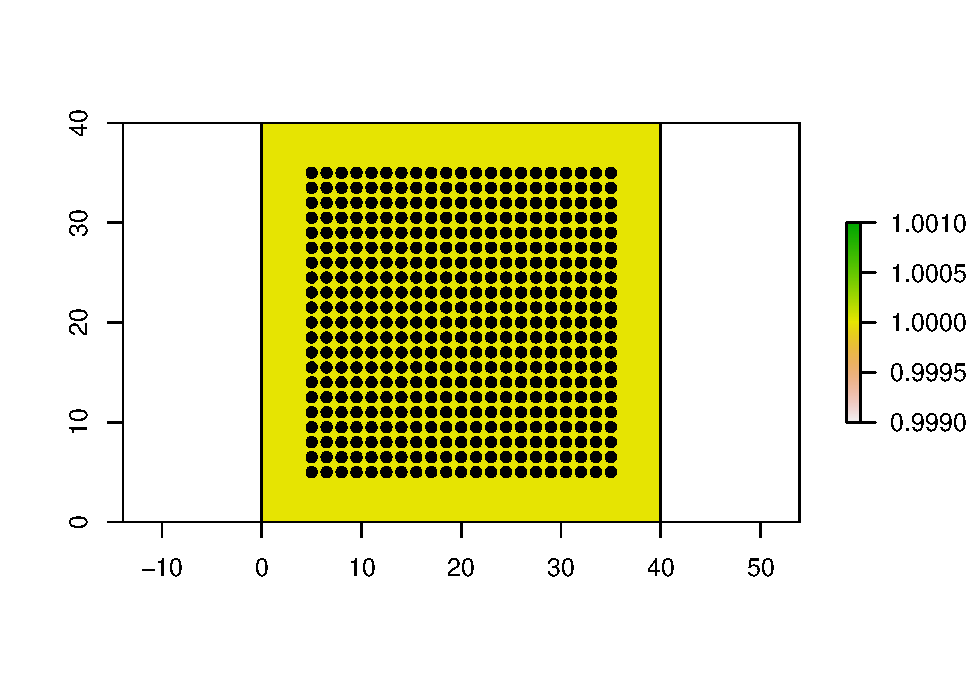
\includegraphics{InterruptionsPDF_files/figure-latex/2-1.pdf}

\begin{Shaded}
\begin{Highlighting}[]
\CommentTok{### ==== 3.SIMULATE INDIVIDUAL STATE MATRIX ===}
\CommentTok{### ====  3.1 DEFINE PHI AND RHO ARRAYS ====  }
\NormalTok{PHI.arr <-}\StringTok{ }\KeywordTok{array}\NormalTok{(}\OtherTok{NA}\NormalTok{, }\KeywordTok{c}\NormalTok{(}\DecValTok{2}\NormalTok{,}\DecValTok{2}\NormalTok{, n.occasions))}
\NormalTok{REPRO.arr <-}\StringTok{ }\KeywordTok{array}\NormalTok{(}\OtherTok{NA}\NormalTok{, }\KeywordTok{c}\NormalTok{(}\DecValTok{2}\NormalTok{,}\DecValTok{2}\NormalTok{, n.occasions))}
\NormalTok{FEC.mat <-}\StringTok{ }\KeywordTok{matrix}\NormalTok{(}\OtherTok{NA}\NormalTok{, }\DataTypeTok{nrow=}\DecValTok{2}\NormalTok{, }\DataTypeTok{ncol=}\NormalTok{n.occasions)}
\NormalTok{phit <-}\StringTok{ }\DecValTok{0}
\NormalTok{fect <-}\StringTok{ }\DecValTok{0}

\ControlFlowTok{for}\NormalTok{(t }\ControlFlowTok{in} \DecValTok{1}\OperatorTok{:}\NormalTok{n.occasions)\{}
   \CommentTok{# DEFINE THE PHI MATRIX}
   \CommentTok{# two states: ALIVE/DEAD}
   \CommentTok{# DRAW PHI FROM NORMAL DISTRIB AND APPLY LOGIT }
\NormalTok{   phit[t]  <-}\StringTok{   }\KeywordTok{inv.logit}\NormalTok{(}\KeywordTok{rnorm}\NormalTok{(}\DecValTok{1}\NormalTok{, }\DataTypeTok{mean=}\KeywordTok{logit}\NormalTok{(phi), }\DataTypeTok{sd=}\NormalTok{sd.phi))}
\NormalTok{   PHI.arr[,,t] <-}\StringTok{  }\KeywordTok{matrix}\NormalTok{(}\KeywordTok{c}\NormalTok{(phit[t]       , }\DecValTok{0}\NormalTok{, }
                             \DecValTok{1}\OperatorTok{-}\NormalTok{phit[t] , }\DecValTok{1}\NormalTok{ ), }\DataTypeTok{ncol=}\DecValTok{2}\NormalTok{, }\DataTypeTok{nrow=}\DecValTok{2}\NormalTok{, }\DataTypeTok{byrow =} \OtherTok{TRUE}\NormalTok{)}
   \CommentTok{# DEFINE REPRO MATRIX (p of reproducing)}
   \CommentTok{# THIS DEFINES THE PROBABILITY OF INDIVIDUALS TO REPRODUCE }
   \CommentTok{# (ASSUME ALL INDIVIDUALS REPRODUCE HERE)}
\NormalTok{   REPRO.arr[,,t] =}\StringTok{ }\KeywordTok{matrix}\NormalTok{(}\KeywordTok{c}\NormalTok{( p.repro, }\DecValTok{0}\NormalTok{,}
                              \DecValTok{0}\NormalTok{      , }\DecValTok{0}\NormalTok{ ), }\DataTypeTok{ncol=}\DecValTok{2}\NormalTok{, }\DataTypeTok{nrow=}\DecValTok{2}\NormalTok{, }\DataTypeTok{byrow =} \OtherTok{TRUE}\NormalTok{)}
   \CommentTok{# DEFINE PER CAPITA RECRUITMENT.}
   \CommentTok{# GIVEN THAT INDIVIDUAL REPRODUCES, HOW MANY ARE RECRUITED}
\NormalTok{   fect[t] <-}\StringTok{   }\KeywordTok{inv.logit}\NormalTok{(}\KeywordTok{rnorm}\NormalTok{(}\DecValTok{1}\NormalTok{, }\DataTypeTok{mean=}\KeywordTok{logit}\NormalTok{(rho), }\DataTypeTok{sd=}\NormalTok{sd.rho))}
\NormalTok{   FEC.mat[,t] =}\StringTok{ }\KeywordTok{c}\NormalTok{(fect[t], }\DecValTok{0}\NormalTok{)}
\NormalTok{\}}

\CommentTok{### ====  3.2 SIMULATE Z ====  }
\NormalTok{z.mx <-}\StringTok{ }\KeywordTok{SimulateZ}\NormalTok{( }\DataTypeTok{N0 =}\NormalTok{ N1,}
                      \DataTypeTok{n.occasions =}\NormalTok{ n.occasions}\DecValTok{-1}\NormalTok{, }
                      \DataTypeTok{PHI =}\NormalTok{ PHI.arr, }
                      \DataTypeTok{REPRO =}\NormalTok{ REPRO.arr, }
                      \DataTypeTok{FEC =}\NormalTok{ FEC.mat, }
                      \DataTypeTok{init.state =} \DecValTok{1}\NormalTok{) }
\NormalTok{myZ <-}\StringTok{ }\NormalTok{z.mx}\OperatorTok{$}\NormalTok{z}
\CommentTok{# ADD THE NOT ENTERED STATE}
\CommentTok{# 1: NOT ENTERERD}
\CommentTok{# 2: ALIVE}
\CommentTok{# 3: DEAD}
\NormalTok{myZ <-}\StringTok{ }\NormalTok{myZ}\OperatorTok{+}\DecValTok{1} 
\NormalTok{myZ[}\KeywordTok{is.na}\NormalTok{(myZ)] <-}\StringTok{ }\DecValTok{1}

\CommentTok{# GET POP COMPOSITION AND PLOT IT}
\NormalTok{z.levels <-}\StringTok{ }\KeywordTok{unique}\NormalTok{(}\KeywordTok{na.omit}\NormalTok{(}\KeywordTok{unlist}\NormalTok{(}\KeywordTok{apply}\NormalTok{(myZ, }\DecValTok{1}\NormalTok{, unique))))  }
\NormalTok{z.levels <-}\StringTok{ }\NormalTok{z.levels[}\KeywordTok{order}\NormalTok{(z.levels)]}
\NormalTok{Pop.Compo <-}\StringTok{ }\KeywordTok{list}\NormalTok{()}
\ControlFlowTok{for}\NormalTok{(l }\ControlFlowTok{in} \DecValTok{1}\OperatorTok{:}\KeywordTok{length}\NormalTok{(z.levels))\{}
\NormalTok{   Pop.Compo[[l]] <-}\StringTok{ }\KeywordTok{apply}\NormalTok{(myZ, }\DecValTok{2}\NormalTok{, }\ControlFlowTok{function}\NormalTok{(x)\{}\KeywordTok{length}\NormalTok{(}\KeywordTok{which}\NormalTok{(x }\OperatorTok{==}\StringTok{ }\NormalTok{z.levels[l]))\})}
\NormalTok{\}}\CommentTok{#l}

\CommentTok{# PLOT CHECK }
\KeywordTok{plot}\NormalTok{(}\DecValTok{1}\OperatorTok{:}\KeywordTok{dim}\NormalTok{(myZ)[}\DecValTok{2}\NormalTok{], Pop.Compo[[}\DecValTok{1}\NormalTok{]], }\DataTypeTok{type=}\StringTok{"l"}\NormalTok{, }\DataTypeTok{col=}\DecValTok{1}\NormalTok{, }\DataTypeTok{lwd=}\DecValTok{2}\NormalTok{,}
     \DataTypeTok{ylim=}\KeywordTok{c}\NormalTok{(}\DecValTok{0}\NormalTok{, }\KeywordTok{max}\NormalTok{(}\KeywordTok{unlist}\NormalTok{(Pop.Compo))), }
     \DataTypeTok{xlab =} \StringTok{"Years"}\NormalTok{, }\DataTypeTok{ylab =} \StringTok{"# of Individuals"}\NormalTok{)}

\ControlFlowTok{for}\NormalTok{(l }\ControlFlowTok{in} \DecValTok{2}\OperatorTok{:}\KeywordTok{length}\NormalTok{(Pop.Compo))\{}
   \KeywordTok{points}\NormalTok{(}\DecValTok{1}\OperatorTok{:}\KeywordTok{dim}\NormalTok{(myZ)[}\DecValTok{2}\NormalTok{],Pop.Compo[[l]], }\DataTypeTok{type=}\StringTok{"l"}\NormalTok{, }\DataTypeTok{col=}\NormalTok{l, }\DataTypeTok{lwd=}\DecValTok{2}\NormalTok{)}
\NormalTok{\}}\CommentTok{#l}
\KeywordTok{legend}\NormalTok{(}\StringTok{"bottomleft"}
\NormalTok{       , }\DataTypeTok{legend =}  \KeywordTok{c}\NormalTok{(}\KeywordTok{unlist}\NormalTok{(}\KeywordTok{lapply}\NormalTok{(z.levels, }\ControlFlowTok{function}\NormalTok{(x)\{}\KeywordTok{paste}\NormalTok{(}\StringTok{" State"}\NormalTok{, x)\})), }\StringTok{"Total"}\NormalTok{)}
\NormalTok{       , }\DataTypeTok{col =} \DecValTok{1}\OperatorTok{:}\KeywordTok{length}\NormalTok{(Pop.Compo)}
\NormalTok{       , }\DataTypeTok{lwd =} \DecValTok{1}
\NormalTok{       , }\DataTypeTok{cex =} \FloatTok{0.6}
\NormalTok{       , }\DataTypeTok{inset =} \FloatTok{0.01}\NormalTok{)}
\end{Highlighting}
\end{Shaded}

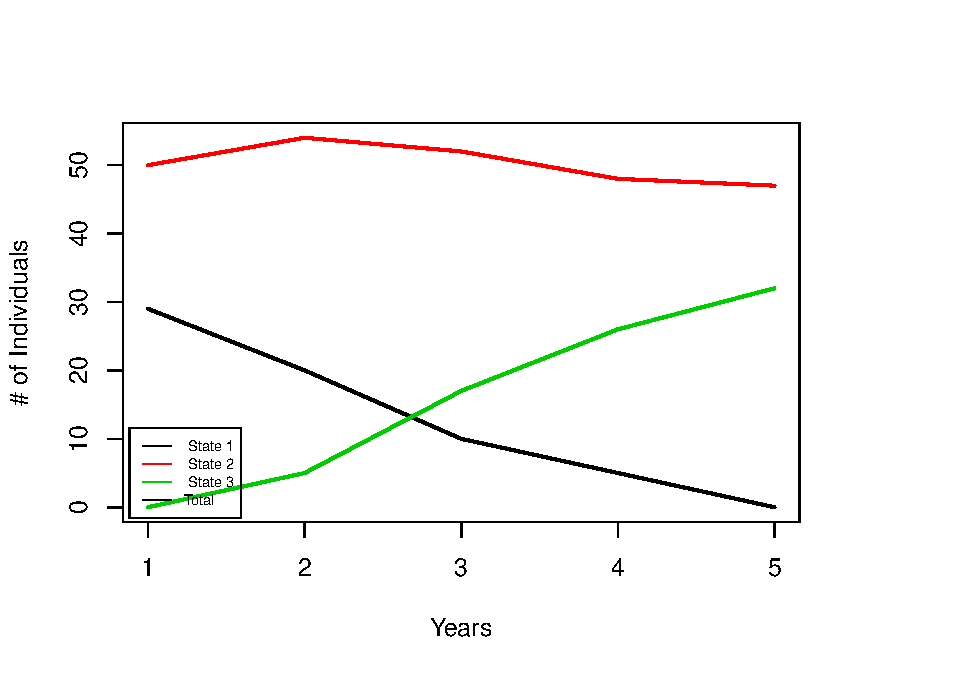
\includegraphics{InterruptionsPDF_files/figure-latex/2-2.pdf}

\begin{Shaded}
\begin{Highlighting}[]
\CommentTok{### ==== 4.SIMULATE INDIVIDUAL AC LOCATIONS ====}
\CommentTok{### ====  4.1 FIRST OCCASION ====}
\CommentTok{# CREATE EMPTY OBJECTS }
\NormalTok{mySimulatedACs <-}\StringTok{ }\KeywordTok{list}\NormalTok{()}
\NormalTok{tempCoords <-}\StringTok{ }\KeywordTok{matrix}\NormalTok{(}\OtherTok{NA}\NormalTok{,}\DataTypeTok{nrow=}\KeywordTok{dim}\NormalTok{(myZ)[}\DecValTok{1}\NormalTok{], }\DataTypeTok{ncol=}\DecValTok{2}\NormalTok{)}

\CommentTok{# SIMULATE UNIFORM LOCATION OF ACS}
\ControlFlowTok{for}\NormalTok{(i }\ControlFlowTok{in} \DecValTok{1}\OperatorTok{:}\KeywordTok{dim}\NormalTok{(myZ)[}\DecValTok{1}\NormalTok{])\{}
\NormalTok{   tempCoords[i,] <-}\StringTok{ }\KeywordTok{rbinomPPSingle}\NormalTok{( }\DataTypeTok{n =} \DecValTok{1}
\NormalTok{                                     , }\DataTypeTok{lowerCoords =}\NormalTok{ lowerCoords}
\NormalTok{                                     , }\DataTypeTok{upperCoords =}\NormalTok{ upperCoords}
\NormalTok{                                     , }\DataTypeTok{intensityWeights =}\NormalTok{ habitatQuality}
\NormalTok{                                     , }\DataTypeTok{areAreas =} \DecValTok{1}
\NormalTok{                                     , }\DataTypeTok{numWindows =} \KeywordTok{nrow}\NormalTok{(lowerCoords))}
\NormalTok{\}}\CommentTok{#i}

\CommentTok{# STORE ACS IN A SP OBJECT}
\NormalTok{mySimulatedACs[[}\DecValTok{1}\NormalTok{]] <-}\StringTok{ }\KeywordTok{SpatialPointsDataFrame}\NormalTok{( tempCoords}
\NormalTok{                                               , }\KeywordTok{data.frame}\NormalTok{( }\DataTypeTok{x =}\NormalTok{ tempCoords[, }\DecValTok{1}\NormalTok{]}
\NormalTok{                                                             , }\DataTypeTok{y =}\NormalTok{ tempCoords[, }\DecValTok{2}\NormalTok{]}
\NormalTok{                                                             , }\DataTypeTok{Id =} \DecValTok{1}\OperatorTok{:}\KeywordTok{nrow}\NormalTok{(tempCoords))}
\NormalTok{                                               , }\DataTypeTok{proj4string =} \KeywordTok{CRS}\NormalTok{(}\KeywordTok{proj4string}\NormalTok{(r)))}
\CommentTok{### ====  4.2 FOLLWOWING YEARS ====}
\CommentTok{# DRAW SUBSEQUENT INDIVIDUAL ACS FROM A NORMAL DISTRIBUTION }
\CommentTok{# CENTERED AROUND THE SOURCE COORDINATE}
\CommentTok{# WITH A SD EQUAL TO "tau"  }
\CommentTok{# THERE IS THE POSSIBILITY TO DEFINE A HABITAT QUALITY SURFACE}
\CommentTok{# FOR THE PUPORSE OF THE STUDY, HABITAT QUALITY WAS UNIFORM (SET TO 1 EVERYWHERE)}
\ControlFlowTok{for}\NormalTok{(t }\ControlFlowTok{in} \DecValTok{2}\OperatorTok{:}\KeywordTok{dim}\NormalTok{(myZ)[}\DecValTok{2}\NormalTok{])\{}
   \ControlFlowTok{for}\NormalTok{(i }\ControlFlowTok{in} \DecValTok{1}\OperatorTok{:}\KeywordTok{nrow}\NormalTok{(tempCoords))\{}
\NormalTok{      tempCoords[i,]  <-}\StringTok{ }\KeywordTok{rbinomMNormSourcePPSingle}\NormalTok{( }\DataTypeTok{n =} \DecValTok{1}
\NormalTok{                                                    , }\DataTypeTok{lowerCoords =}\NormalTok{ lowerCoords}
\NormalTok{                                                    , }\DataTypeTok{upperCoords =}\NormalTok{ upperCoords}
\NormalTok{                                                    , }\DataTypeTok{sourceCoords =}\NormalTok{ tempCoords[i,]}
\NormalTok{                                                    , }\DataTypeTok{normSD =}\NormalTok{ tau}
\NormalTok{                                                    , }\DataTypeTok{intensityWeights =}\NormalTok{ habitatQuality}
\NormalTok{                                                    , }\DataTypeTok{areAreas =} \DecValTok{1}
\NormalTok{                                                    , }\DataTypeTok{numWindows =} \KeywordTok{nrow}\NormalTok{(lowerCoords))}
\NormalTok{   \}}
   \CommentTok{# STORE ACS IN A SP OBJECT}
\NormalTok{   mySimulatedACs[[t]] <-}\StringTok{ }\KeywordTok{SpatialPointsDataFrame}\NormalTok{(}
\NormalTok{                            tempCoords}
\NormalTok{                            , }\KeywordTok{data.frame}\NormalTok{( }\DataTypeTok{x =}\NormalTok{ tempCoords[, }\DecValTok{1}\NormalTok{]}
\NormalTok{                                         , }\DataTypeTok{y =}\NormalTok{ tempCoords[, }\DecValTok{2}\NormalTok{]}
\NormalTok{                                         , }\DataTypeTok{Id =} \DecValTok{1}\OperatorTok{:}\KeywordTok{nrow}\NormalTok{(tempCoords))}
\NormalTok{                            , }\DataTypeTok{proj4string =} 
                              \KeywordTok{CRS}\NormalTok{(}\KeywordTok{proj4string}\NormalTok{(mySimulatedACs[[t}\DecValTok{-1}\NormalTok{]])))}
\NormalTok{\}}\CommentTok{#t}

\CommentTok{# PLOT CHECK}
\KeywordTok{plot}\NormalTok{(}\KeywordTok{aggregate}\NormalTok{(}\KeywordTok{rasterToPolygons}\NormalTok{(r,}\DataTypeTok{fun =} \ControlFlowTok{function}\NormalTok{(x)\{x}\OperatorTok{>}\DecValTok{0}\NormalTok{\})))}
\KeywordTok{points}\NormalTok{(detectors.sp, }\DataTypeTok{pch=}\DecValTok{16}\NormalTok{, }\DataTypeTok{cex=}\FloatTok{0.5}\NormalTok{)}
\NormalTok{col <-}\StringTok{ }\KeywordTok{rainbow}\NormalTok{(}\KeywordTok{length}\NormalTok{(mySimulatedACs[[}\DecValTok{1}\NormalTok{]]))}
\KeywordTok{points}\NormalTok{(mySimulatedACs[[}\DecValTok{1}\NormalTok{]], }\DataTypeTok{pch=}\DecValTok{21}\NormalTok{, }\DataTypeTok{bg=}\NormalTok{col)}

\ControlFlowTok{for}\NormalTok{(t }\ControlFlowTok{in} \DecValTok{2}\OperatorTok{:}\KeywordTok{length}\NormalTok{(mySimulatedACs))\{}
   \KeywordTok{points}\NormalTok{(mySimulatedACs[[t]], }\DataTypeTok{pch=}\DecValTok{21}\NormalTok{, }\DataTypeTok{bg=}\NormalTok{col)}
   \KeywordTok{arrows}\NormalTok{( }\DataTypeTok{x0 =} \KeywordTok{coordinates}\NormalTok{(mySimulatedACs[[t]])[ ,}\DecValTok{1}\NormalTok{]}
\NormalTok{           , }\DataTypeTok{x1 =} \KeywordTok{coordinates}\NormalTok{(mySimulatedACs[[t}\DecValTok{-1}\NormalTok{]])[ ,}\DecValTok{1}\NormalTok{]}
\NormalTok{           , }\DataTypeTok{y0 =} \KeywordTok{coordinates}\NormalTok{(mySimulatedACs[[t]])[ ,}\DecValTok{2}\NormalTok{]}
\NormalTok{           , }\DataTypeTok{y1 =} \KeywordTok{coordinates}\NormalTok{(mySimulatedACs[[t}\DecValTok{-1}\NormalTok{]])[ ,}\DecValTok{2}\NormalTok{], }\DataTypeTok{col =}\NormalTok{ col, }\DataTypeTok{length =} \FloatTok{0.08}\NormalTok{)}
\NormalTok{\}}\CommentTok{#t}
\end{Highlighting}
\end{Shaded}

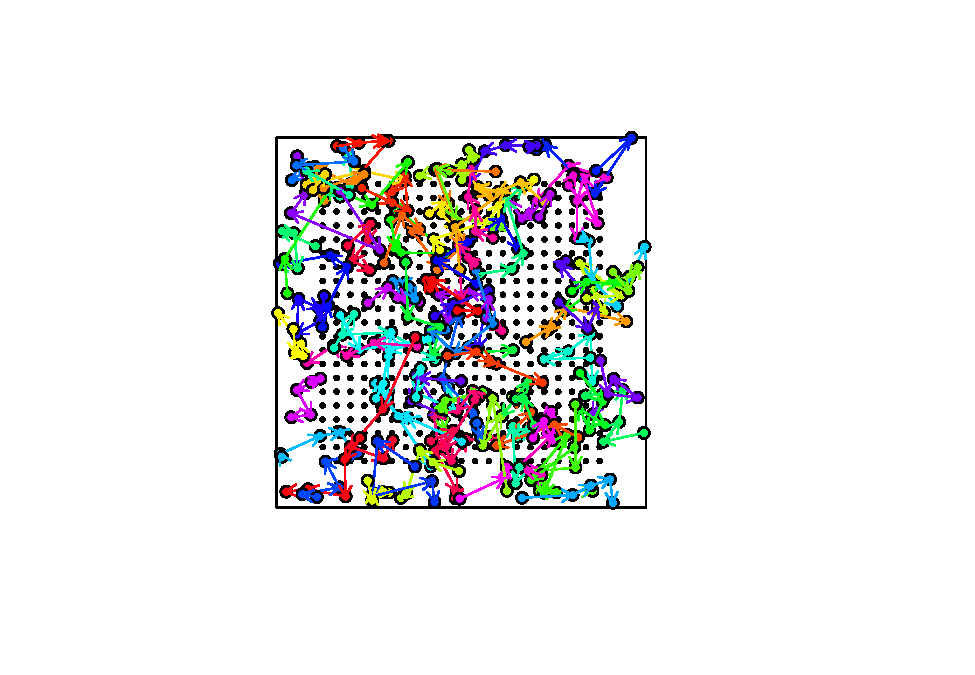
\includegraphics{InterruptionsPDF_files/figure-latex/2-3.pdf}

\begin{Shaded}
\begin{Highlighting}[]
\CommentTok{### ==== 5.SIMULATE DETECTION ====}
\CommentTok{### ====  5.1 DETECTION ARRAY ====}
\NormalTok{z.not.alive <-}\StringTok{ }\KeywordTok{apply}\NormalTok{(myZ, }\DecValTok{2}\NormalTok{, }\ControlFlowTok{function}\NormalTok{(x)\{}\KeywordTok{which}\NormalTok{(x }\OperatorTok\StringTok{ }\KeywordTok{c}\NormalTok{(}\DecValTok{1}\NormalTok{,}\DecValTok{3}\NormalTok{))\})}
\NormalTok{Y <-}\StringTok{ }\KeywordTok{array}\NormalTok{(}\OtherTok{NA}\NormalTok{, }\KeywordTok{c}\NormalTok{(}\KeywordTok{dim}\NormalTok{(myZ)[}\DecValTok{1}\NormalTok{], }\KeywordTok{length}\NormalTok{(detectors.sp), }\KeywordTok{dim}\NormalTok{(myZ)[}\DecValTok{2}\NormalTok{]))}

\ControlFlowTok{for}\NormalTok{(t }\ControlFlowTok{in} \DecValTok{1}\OperatorTok{:}\KeywordTok{dim}\NormalTok{(myZ)[}\DecValTok{2}\NormalTok{])\{}
\NormalTok{   D <-}\StringTok{ }\KeywordTok{gDistance}\NormalTok{(detectors.sp, mySimulatedACs[[t]], }\DataTypeTok{byid=}\OtherTok{TRUE}\NormalTok{)}
   \CommentTok{# OBTAIN Y DETECTION MATRIX USING HALF NORMAL DETECTION FUNCTION (EQN 7 IN MAIN TEXT)}
\NormalTok{   fixed.effects <-}\StringTok{ }\KeywordTok{rep}\NormalTok{(}\KeywordTok{log}\NormalTok{(p0), }\KeywordTok{length}\NormalTok{(detectors.sp))}
\NormalTok{   pzero <-}\StringTok{ }\KeywordTok{exp}\NormalTok{(fixed.effects)}
\NormalTok{   p <-}\StringTok{ }\NormalTok{pzero }\OperatorTok{*}\StringTok{ }\KeywordTok{exp}\NormalTok{(}\OperatorTok{-}\NormalTok{D}\OperatorTok{*}\NormalTok{D}\OperatorTok{/}\NormalTok{(}\DecValTok{2}\OperatorTok{*}\NormalTok{sigma}\OperatorTok{*}\NormalTok{sigma))}
\NormalTok{   Y[,,t] <-}\StringTok{ }\KeywordTok{apply}\NormalTok{(p, }\KeywordTok{c}\NormalTok{(}\DecValTok{1}\NormalTok{,}\DecValTok{2}\NormalTok{), }\ControlFlowTok{function}\NormalTok{(x) }\KeywordTok{rbinom}\NormalTok{(}\DecValTok{1}\NormalTok{, }\DecValTok{1}\NormalTok{, x))}
   \CommentTok{# individuals not alive can't be detected}
\NormalTok{   Y[z.not.alive[[t]],,t] <-}\StringTok{ }\DecValTok{0}
   
\NormalTok{\}}\CommentTok{#t}
\CommentTok{### ====  5.1 PLOT CHECK ====}
\KeywordTok{par}\NormalTok{(}\DataTypeTok{mfrow=}\KeywordTok{c}\NormalTok{(}\DecValTok{2}\NormalTok{,}\DecValTok{3}\NormalTok{), }\DataTypeTok{mar=}\KeywordTok{c}\NormalTok{(}\DecValTok{0}\NormalTok{,}\DecValTok{0}\NormalTok{,}\DecValTok{3}\NormalTok{,}\DecValTok{0}\NormalTok{))}
\ControlFlowTok{for}\NormalTok{(t }\ControlFlowTok{in} \DecValTok{1}\OperatorTok{:}\KeywordTok{dim}\NormalTok{(myZ)[}\DecValTok{2}\NormalTok{])\{}
   \KeywordTok{plot}\NormalTok{(myStudyArea)}
   \KeywordTok{title}\NormalTok{(t)}
   \KeywordTok{points}\NormalTok{(detectors.sp, }\DataTypeTok{pch=}\DecValTok{16}\NormalTok{, }\DataTypeTok{cex=}\FloatTok{0.6}\NormalTok{) }
\NormalTok{   detections <-}\StringTok{ }\KeywordTok{apply}\NormalTok{(Y[,,t],}\DecValTok{1}\NormalTok{, }\ControlFlowTok{function}\NormalTok{(x) }\KeywordTok{which}\NormalTok{(x}\OperatorTok{>}\DecValTok{0}\NormalTok{))}
\NormalTok{   col <-}\StringTok{ }\KeywordTok{rainbow}\NormalTok{(}\KeywordTok{dim}\NormalTok{(Y)[}\DecValTok{1}\NormalTok{])[}\KeywordTok{sample}\NormalTok{(}\KeywordTok{dim}\NormalTok{(Y)[}\DecValTok{1}\NormalTok{])]}
   \ControlFlowTok{for}\NormalTok{(i }\ControlFlowTok{in} \DecValTok{1}\OperatorTok{:}\KeywordTok{length}\NormalTok{(detections))\{}
      \ControlFlowTok{if}\NormalTok{(}\OperatorTok{!}\NormalTok{i }\OperatorTok\StringTok{ }\NormalTok{z.not.alive[[t]])\{}
         \ControlFlowTok{if}\NormalTok{(}\KeywordTok{length}\NormalTok{(detectors.sp[detections[[i]],])}\OperatorTok{==}\DecValTok{0}\NormalTok{)\{}
            \KeywordTok{points}\NormalTok{(mySimulatedACs[[t]][i,],}\DataTypeTok{bg=}\NormalTok{col[i], }\DataTypeTok{pch=}\DecValTok{21}\NormalTok{, }\DataTypeTok{cex=}\FloatTok{0.5}\NormalTok{)}
            \KeywordTok{points}\NormalTok{(mySimulatedACs[[t]][i,], }\DataTypeTok{col=}\NormalTok{col[i], }\DataTypeTok{pch=}\DecValTok{4}\NormalTok{)}
            
\NormalTok{         \}}\ControlFlowTok{else}\NormalTok{\{}
            \KeywordTok{points}\NormalTok{(detectors.sp[detections[[i]],],}\DataTypeTok{col=}\NormalTok{col[i], }\DataTypeTok{pch=}\DecValTok{16}\NormalTok{, }\DataTypeTok{cex=}\FloatTok{0.7}\NormalTok{)}
\NormalTok{            ac <-}\StringTok{ }\KeywordTok{coordinates}\NormalTok{(mySimulatedACs[[t]][i,])}
\NormalTok{            dets <-}\StringTok{ }\KeywordTok{coordinates}\NormalTok{(detectors.sp[detections[[i]],])}
            \KeywordTok{segments}\NormalTok{(}\DataTypeTok{x0=}\NormalTok{ac[}\DecValTok{1}\NormalTok{,}\DecValTok{1}\NormalTok{], }\DataTypeTok{x1=}\NormalTok{dets[,}\DecValTok{1}\NormalTok{] , }\DataTypeTok{y0=}\NormalTok{ac[}\DecValTok{1}\NormalTok{,}\DecValTok{2}\NormalTok{], }\DataTypeTok{y1=}\NormalTok{dets[,}\DecValTok{2}\NormalTok{], }\DataTypeTok{col=}\NormalTok{col[i])}
            \KeywordTok{points}\NormalTok{(mySimulatedACs[[t]][i,],}\DataTypeTok{bg=}\NormalTok{col[i], }\DataTypeTok{pch=}\DecValTok{21}\NormalTok{)}
            
\NormalTok{         \}}\CommentTok{#else}
\NormalTok{      \}}\CommentTok{#if}
\NormalTok{   \}}\CommentTok{#i   }
\NormalTok{\}}\CommentTok{#t}

\CommentTok{### ==== 6.AUGMENT DATA SET ====}
\CommentTok{# REMOVE UNDETECTED IDS}
\NormalTok{detected.time <-}\StringTok{ }\KeywordTok{apply}\NormalTok{(Y, }\KeywordTok{c}\NormalTok{(}\DecValTok{1}\NormalTok{,}\DecValTok{3}\NormalTok{), }\ControlFlowTok{function}\NormalTok{(x) }\KeywordTok{any}\NormalTok{(x }\OperatorTok{>=}\StringTok{ }\DecValTok{1}\NormalTok{))}
\NormalTok{detected <-}\StringTok{ }\KeywordTok{apply}\NormalTok{(detected.time, }\KeywordTok{c}\NormalTok{(}\DecValTok{1}\NormalTok{), }\ControlFlowTok{function}\NormalTok{(x) }\KeywordTok{sum}\NormalTok{(x}\OperatorTok{==}\DecValTok{1}\NormalTok{)}\OperatorTok{>}\DecValTok{0}\NormalTok{)}
\NormalTok{Y <-}\StringTok{ }\NormalTok{Y[detected,,]}

\CommentTok{#AUGMENTATION=  "augmentation" x N OF THE SUPER POPULATION}
\NormalTok{y.aug <-}\StringTok{ }\KeywordTok{array}\NormalTok{(}\DecValTok{0}\NormalTok{,}\KeywordTok{c}\NormalTok{(  }\KeywordTok{nrow}\NormalTok{(myZ)}\OperatorTok{*}\NormalTok{augmentation }\OperatorTok{-}\StringTok{ }\KeywordTok{dim}\NormalTok{(Y)[}\DecValTok{1}\NormalTok{] ,}\KeywordTok{dim}\NormalTok{(Y)[}\DecValTok{2}\OperatorTok{:}\DecValTok{3}\NormalTok{]))}
\NormalTok{y <-}\StringTok{ }\KeywordTok{abind}\NormalTok{(Y , y.aug, }\DataTypeTok{along =} \DecValTok{1}\NormalTok{)}
\KeywordTok{dim}\NormalTok{(y)}
\end{Highlighting}
\end{Shaded}

\begin{verbatim}
## [1] 123 441   5
\end{verbatim}

\begin{Shaded}
\begin{Highlighting}[]
\CommentTok{### ==== 7.ADD INTERUPTION ====}
\NormalTok{interuptions <-}\StringTok{ }\KeywordTok{which}\NormalTok{(toggle.interuption}\OperatorTok{==}\DecValTok{0}\NormalTok{)}
\ControlFlowTok{if}\NormalTok{(}\KeywordTok{length}\NormalTok{(interuptions)}\OperatorTok{>}\DecValTok{0}\NormalTok{)\{}
   \CommentTok{# ZERO DETECTIONS DURING INTERUPTIONS}
\NormalTok{   y[,,interuptions] <-}\StringTok{ }\DecValTok{0}
\NormalTok{\}}

\CommentTok{### ==== 8.RECONSTRUCT z VALUES ====}
\NormalTok{z <-}\StringTok{ }\KeywordTok{apply}\NormalTok{(y, }\KeywordTok{c}\NormalTok{(}\DecValTok{1}\NormalTok{,}\DecValTok{3}\NormalTok{), }\ControlFlowTok{function}\NormalTok{(x) }\KeywordTok{any}\NormalTok{(x}\OperatorTok{>}\DecValTok{0}\NormalTok{))}
\NormalTok{z <-}\StringTok{ }\KeywordTok{ifelse}\NormalTok{(z, }\DecValTok{2}\NormalTok{, }\OtherTok{NA}\NormalTok{)}

\NormalTok{z <-}\StringTok{ }\KeywordTok{t}\NormalTok{(}\KeywordTok{apply}\NormalTok{(z, }\DecValTok{1}\NormalTok{, }\ControlFlowTok{function}\NormalTok{(zz)\{}
   \ControlFlowTok{if}\NormalTok{(}\KeywordTok{any}\NormalTok{(}\OperatorTok{!}\KeywordTok{is.na}\NormalTok{(zz)))\{}
\NormalTok{      range.det <-}\StringTok{ }\KeywordTok{range}\NormalTok{(}\KeywordTok{which}\NormalTok{(}\OperatorTok{!}\KeywordTok{is.na}\NormalTok{(zz)))}
\NormalTok{      zz[range.det[}\DecValTok{1}\NormalTok{]}\OperatorTok{:}\NormalTok{range.det[}\DecValTok{2}\NormalTok{]] <-}\StringTok{ }\DecValTok{2}
\NormalTok{   \}}
   \KeywordTok{return}\NormalTok{(zz)}
\NormalTok{\}))}

\CommentTok{### ==== 9.GENERATE z INITIAL values====}
\NormalTok{z.init <-}\StringTok{ }\KeywordTok{t}\NormalTok{(}\KeywordTok{apply}\NormalTok{(z, }\DecValTok{1}\NormalTok{, }\ControlFlowTok{function}\NormalTok{(zz)\{}
\NormalTok{   out <-}\StringTok{ }\NormalTok{zz}
\NormalTok{   out[] <-}\StringTok{ }\DecValTok{1}
   \ControlFlowTok{if}\NormalTok{(}\KeywordTok{any}\NormalTok{(}\OperatorTok{!}\KeywordTok{is.na}\NormalTok{(zz)))\{}
\NormalTok{      range.det <-}\StringTok{ }\KeywordTok{range}\NormalTok{(}\KeywordTok{which}\NormalTok{(}\OperatorTok{!}\KeywordTok{is.na}\NormalTok{(zz)))}
      \ControlFlowTok{if}\NormalTok{(range.det[}\DecValTok{1}\NormalTok{]}\OperatorTok{>}\DecValTok{1}\NormalTok{)zz[}\DecValTok{1}\OperatorTok{:}\NormalTok{(range.det[}\DecValTok{1}\NormalTok{]}\OperatorTok{-}\DecValTok{1}\NormalTok{)] <-}\StringTok{ }\DecValTok{1}
      \ControlFlowTok{if}\NormalTok{(range.det[}\DecValTok{2}\NormalTok{]}\OperatorTok{<}\KeywordTok{length}\NormalTok{(zz))zz[(range.det[}\DecValTok{2}\NormalTok{]}\OperatorTok{+}\DecValTok{1}\NormalTok{)}\OperatorTok{:}\KeywordTok{length}\NormalTok{(zz)] <-}\StringTok{ }\DecValTok{3}
\NormalTok{      out[] <-}\StringTok{ }\NormalTok{zz}
\NormalTok{   \} }
   \KeywordTok{return}\NormalTok{(out)}
\NormalTok{\}))}

\NormalTok{z.init <-}\StringTok{ }\KeywordTok{ifelse}\NormalTok{(}\OperatorTok{!}\KeywordTok{is.na}\NormalTok{(z), }\OtherTok{NA}\NormalTok{, z.init)}
\end{Highlighting}
\end{Shaded}

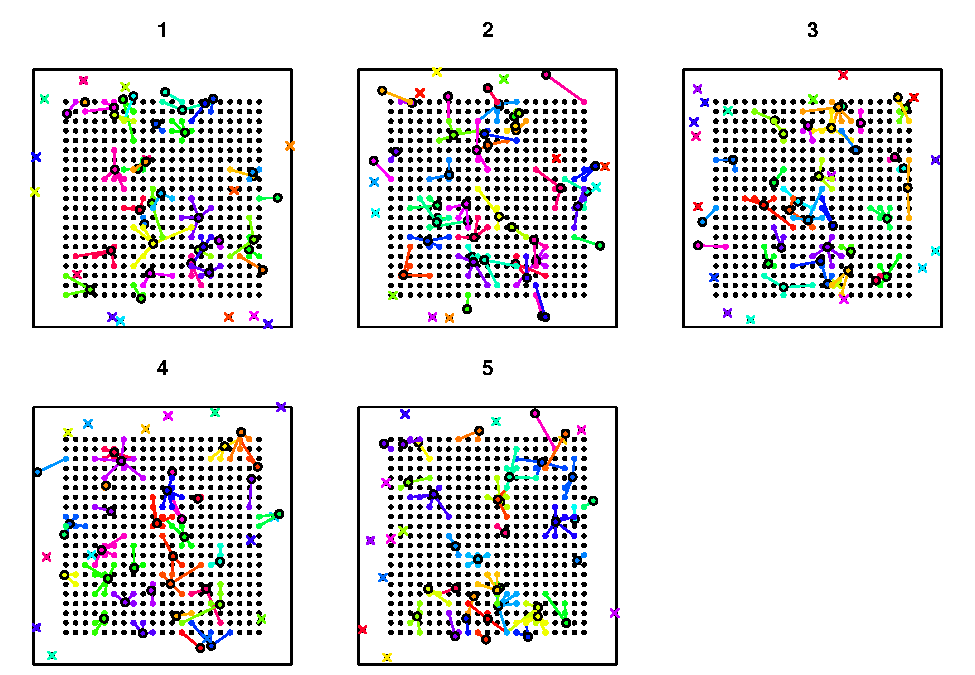
\includegraphics{InterruptionsPDF_files/figure-latex/2-4.pdf}

\hypertarget{iii.nimble}{%
\subsection{III.NIMBLE}\label{iii.nimble}}

\begin{Shaded}
\begin{Highlighting}[]
\CommentTok{### ==== 1.MODEL CODE ==== }
\NormalTok{modelCode <-}\StringTok{ }\KeywordTok{nimbleCode}\NormalTok{(\{}
  \CommentTok{##--------------------------------------------------------------------------------}
  \CommentTok{##-----------------------------## }
  \CommentTok{##------ SPATIAL PROCESS ------##  }
  \CommentTok{##-----------------------------##  }
\NormalTok{  tau }\OperatorTok{~}\StringTok{ }\KeywordTok{dgamma}\NormalTok{(}\FloatTok{0.001}\NormalTok{, }\FloatTok{0.001}\NormalTok{)}
  
  \ControlFlowTok{for}\NormalTok{(i }\ControlFlowTok{in} \DecValTok{1}\OperatorTok{:}\NormalTok{n.individuals)\{}
\NormalTok{    sxy[i, }\DecValTok{1}\OperatorTok{:}\DecValTok{2}\NormalTok{, }\DecValTok{1}\NormalTok{] }\OperatorTok{~}\StringTok{ }\KeywordTok{dbinomPPSingle}\NormalTok{(lowerHabCoords[}\DecValTok{1}\OperatorTok{:}\NormalTok{n.cells, }\DecValTok{1}\OperatorTok{:}\DecValTok{2}\NormalTok{]}
\NormalTok{                                    , upperHabCoords[}\DecValTok{1}\OperatorTok{:}\NormalTok{n.cells, }\DecValTok{1}\OperatorTok{:}\DecValTok{2}\NormalTok{],}
\NormalTok{                                    mu[}\DecValTok{1}\OperatorTok{:}\NormalTok{n.cells], }\DecValTok{1}\NormalTok{, n.cells)}
    \ControlFlowTok{for}\NormalTok{(t }\ControlFlowTok{in} \DecValTok{2}\OperatorTok{:}\NormalTok{n.years)\{}
\NormalTok{      sxy[i, }\DecValTok{1}\OperatorTok{:}\DecValTok{2}\NormalTok{, t] }\OperatorTok{~}\StringTok{ }\KeywordTok{dbinomMNormSourcePPSingle}\NormalTok{(lowerHabCoords[}\DecValTok{1}\OperatorTok{:}\NormalTok{n.cells, }\DecValTok{1}\OperatorTok{:}\DecValTok{2}\NormalTok{]}
\NormalTok{                                                 , upperHabCoords[}\DecValTok{1}\OperatorTok{:}\NormalTok{n.cells, }\DecValTok{1}\OperatorTok{:}\DecValTok{2}\NormalTok{]}
\NormalTok{                                                 , sxy[i, }\DecValTok{1}\OperatorTok{:}\DecValTok{2}\NormalTok{, t }\OperatorTok{-}\StringTok{ }\DecValTok{1}\NormalTok{]}
\NormalTok{                                                 , tau}
\NormalTok{                                                 , mu[}\DecValTok{1}\OperatorTok{:}\NormalTok{n.cells]}
\NormalTok{                                                 , }\DecValTok{1}
\NormalTok{                                                 , n.cells,}\OperatorTok{-}\DecValTok{1}\NormalTok{)}

\NormalTok{    \}}\CommentTok{#t}
\NormalTok{  \}}\CommentTok{#i}

  
  \CommentTok{##--------------------------------------------------------------------------------}
  \CommentTok{##-------------------------------## }
  \CommentTok{##----- DEMOGRAPHIC PROCESS -----## }
  \CommentTok{##-------------------------------##     }
\NormalTok{  psi }\OperatorTok{~}\StringTok{ }\KeywordTok{dunif}\NormalTok{(}\DecValTok{0}\NormalTok{, }\DecValTok{1}\NormalTok{)}
\NormalTok{  phi }\OperatorTok{~}\StringTok{ }\KeywordTok{dunif}\NormalTok{(}\DecValTok{0}\NormalTok{, }\DecValTok{1}\NormalTok{)}
\NormalTok{  rho }\OperatorTok{~}\StringTok{ }\KeywordTok{dunif}\NormalTok{(}\DecValTok{0}\NormalTok{, }\DecValTok{5}\NormalTok{)}
  \ControlFlowTok{for}\NormalTok{ (t }\ControlFlowTok{in} \DecValTok{2}\OperatorTok{:}\NormalTok{n.years) \{}
\NormalTok{    gamma[t }\OperatorTok{-}\StringTok{ }\DecValTok{1}\NormalTok{] <-}\StringTok{ }\NormalTok{(N[t }\OperatorTok{-}\StringTok{ }\DecValTok{1}\NormalTok{] }\OperatorTok{*}\StringTok{ }\NormalTok{rho)}\OperatorTok{/}\NormalTok{n.available[t }\OperatorTok{-}\StringTok{ }\DecValTok{1}\NormalTok{]}
\NormalTok{  \} }\CommentTok{#t}
\NormalTok{  omeg1[}\DecValTok{1}\NormalTok{] <-}\StringTok{ }\DecValTok{1} \OperatorTok{-}\StringTok{ }\NormalTok{psi}
\NormalTok{  omeg1[}\DecValTok{2}\NormalTok{] <-}\StringTok{ }\NormalTok{psi}
\NormalTok{  omeg1[}\DecValTok{3}\NormalTok{] <-}\StringTok{ }\DecValTok{0}
  \ControlFlowTok{for}\NormalTok{ (t }\ControlFlowTok{in} \DecValTok{1}\OperatorTok{:}\NormalTok{(nyears1)) \{}
    \CommentTok{# NOT ENTERED}
\NormalTok{    omega[}\DecValTok{1}\NormalTok{, }\DecValTok{1}\NormalTok{, t] <-}\StringTok{ }\DecValTok{1} \OperatorTok{-}\StringTok{ }\NormalTok{gamma[t]}
\NormalTok{    omega[}\DecValTok{1}\NormalTok{, }\DecValTok{2}\NormalTok{, t] <-}\StringTok{ }\NormalTok{gamma[t]}
\NormalTok{    omega[}\DecValTok{1}\NormalTok{, }\DecValTok{3}\NormalTok{, t] <-}\StringTok{ }\DecValTok{0}
    \CommentTok{# ALIVE}
\NormalTok{    omega[}\DecValTok{2}\NormalTok{, }\DecValTok{1}\NormalTok{, t] <-}\StringTok{ }\DecValTok{0}
\NormalTok{    omega[}\DecValTok{2}\NormalTok{, }\DecValTok{2}\NormalTok{, t] <-}\StringTok{ }\NormalTok{phi}
\NormalTok{    omega[}\DecValTok{2}\NormalTok{, }\DecValTok{3}\NormalTok{, t] <-}\StringTok{ }\DecValTok{1} \OperatorTok{-}\StringTok{ }\NormalTok{phi}
    \CommentTok{# DEAD}
\NormalTok{    omega[}\DecValTok{3}\NormalTok{, }\DecValTok{1}\NormalTok{, t] <-}\StringTok{ }\DecValTok{0}
\NormalTok{    omega[}\DecValTok{3}\NormalTok{, }\DecValTok{2}\NormalTok{, t] <-}\StringTok{ }\DecValTok{0}
\NormalTok{    omega[}\DecValTok{3}\NormalTok{, }\DecValTok{3}\NormalTok{, t] <-}\StringTok{ }\DecValTok{1}
\NormalTok{  \} }\CommentTok{#t}
  \ControlFlowTok{for}\NormalTok{ (i }\ControlFlowTok{in} \DecValTok{1}\OperatorTok{:}\NormalTok{n.individuals) \{}
\NormalTok{    z[i, }\DecValTok{1}\NormalTok{] }\OperatorTok{~}\StringTok{ }\KeywordTok{dcat}\NormalTok{(omeg1[}\DecValTok{1}\OperatorTok{:}\DecValTok{3}\NormalTok{])}
    \ControlFlowTok{for}\NormalTok{ (t }\ControlFlowTok{in} \DecValTok{1}\OperatorTok{:}\NormalTok{(nyears1)) \{}
\NormalTok{      z[i, t }\OperatorTok{+}\StringTok{ }\DecValTok{1}\NormalTok{] }\OperatorTok{~}\StringTok{ }\KeywordTok{dcat}\NormalTok{(omega[z[i, t], }\DecValTok{1}\OperatorTok{:}\DecValTok{3}\NormalTok{, t])}
\NormalTok{    \} }\CommentTok{#t}
\NormalTok{  \}}
  
  \CommentTok{##--------------------------------------------------------------------------------   }
  \CommentTok{##-----------------------------##}
  \CommentTok{##----- DETECTION PROCESS -----## }
  \CommentTok{##-----------------------------## }
\NormalTok{  sigma }\OperatorTok{~}\StringTok{ }\KeywordTok{dunif}\NormalTok{(}\DecValTok{0}\NormalTok{,}\DecValTok{5}\NormalTok{)}
\NormalTok{  p0 }\OperatorTok{~}\StringTok{ }\KeywordTok{dunif}\NormalTok{(}\DecValTok{0}\NormalTok{,}\DecValTok{1}\NormalTok{)}
  \ControlFlowTok{for}\NormalTok{(i }\ControlFlowTok{in} \DecValTok{1}\OperatorTok{:}\StringTok{ }\NormalTok{n.individuals)\{}
    \ControlFlowTok{for}\NormalTok{(t }\ControlFlowTok{in} \DecValTok{1}\OperatorTok{:}\NormalTok{n.years)\{}
\NormalTok{      y[i,}\DecValTok{1}\OperatorTok{:}\NormalTok{nMaxDetectors,t] }\OperatorTok{~}\StringTok{ }\KeywordTok{dbin_LESSCachedAllSparse}\NormalTok{(}
             \DataTypeTok{pZero =}\NormalTok{ p0 }\OperatorTok{*}\StringTok{ }\NormalTok{toggle[t]}
\NormalTok{            , }\DataTypeTok{sxy =}\NormalTok{ sxy[i,}\DecValTok{1}\OperatorTok{:}\DecValTok{2}\NormalTok{,t]}
\NormalTok{            , }\DataTypeTok{sigma =}\NormalTok{ sigma}
\NormalTok{            , nbDetections[i,t]}
\NormalTok{            , }\DataTypeTok{yDets =}\NormalTok{ yDets[i,}\DecValTok{1}\OperatorTok{:}\NormalTok{nMaxDetectors,t]}
\NormalTok{            , }\DataTypeTok{detector.xy =}\NormalTok{  detector.xy[}\DecValTok{1}\OperatorTok{:}\NormalTok{n.detectors,}\DecValTok{1}\OperatorTok{:}\DecValTok{2}\NormalTok{]}
\NormalTok{            , }\DataTypeTok{trials =}\NormalTok{ trials[}\DecValTok{1}\OperatorTok{:}\NormalTok{n.detectors]}
\NormalTok{            , }\DataTypeTok{detectorIndex =}\NormalTok{ detectorIndex[}\DecValTok{1}\OperatorTok{:}\NormalTok{n.cellsSparse,}\DecValTok{1}\OperatorTok{:}\NormalTok{maxNBDets]}
\NormalTok{            , }\DataTypeTok{nDetectorsLESS =}\NormalTok{ nDetectorsLESS[}\DecValTok{1}\OperatorTok{:}\NormalTok{n.cellsSparse]}
\NormalTok{            , }\DataTypeTok{ResizeFactor =}\NormalTok{ ResizeFactor}
\NormalTok{            , }\DataTypeTok{maxNBDets =}\NormalTok{ maxNBDets}
\NormalTok{            , }\DataTypeTok{habitatID =}\NormalTok{ habitatIDDet[}\DecValTok{1}\OperatorTok{:}\NormalTok{y.maxDet,}\DecValTok{1}\OperatorTok{:}\NormalTok{x.maxDet]}
\NormalTok{            , }\DataTypeTok{maxDist =}\NormalTok{ maxDist}
\NormalTok{            , }\DataTypeTok{indicator =}\NormalTok{ z[i,t]}\OperatorTok{==}\DecValTok{2}\NormalTok{)}
\NormalTok{    \}}\CommentTok{#t}
\NormalTok{  \}}\CommentTok{#i}

  
  \CommentTok{##----------------------------------------------------------------------------------------------                                        }
  \CommentTok{##----------------------------------------## }
  \CommentTok{##---------- DERIVED PARAMETERS ----------##}
  \CommentTok{##----------------------------------------##}
  \ControlFlowTok{for}\NormalTok{(t }\ControlFlowTok{in} \DecValTok{1}\OperatorTok{:}\NormalTok{n.years)\{}
\NormalTok{    N[t] <-}\StringTok{ }\KeywordTok{sum}\NormalTok{(z[}\DecValTok{1}\OperatorTok{:}\NormalTok{n.individuals, t]}\OperatorTok{==}\DecValTok{2}\NormalTok{) }
\NormalTok{    n.available[t] <-}\StringTok{ }\KeywordTok{sum}\NormalTok{(z[}\DecValTok{1}\OperatorTok{:}\NormalTok{n.individuals, t]}\OperatorTok{==}\DecValTok{1}\NormalTok{)}
\NormalTok{  \}}\CommentTok{#t}
\NormalTok{\}) }

\CommentTok{### ==== 2.NIMBLE DATA ====  }
\NormalTok{nimDims <-}\StringTok{ }\KeywordTok{list}\NormalTok{(  }\StringTok{"omeg1"}\NormalTok{ =}\StringTok{ }\DecValTok{3}
\NormalTok{                  , }\StringTok{"omega"}\NormalTok{ =}\StringTok{ }\KeywordTok{c}\NormalTok{(}\DecValTok{3}\NormalTok{,}\DecValTok{3}\NormalTok{,}\DecValTok{4}\NormalTok{)}
\NormalTok{                  , }\StringTok{"z"}\NormalTok{ =}\StringTok{ }\KeywordTok{c}\NormalTok{(}\KeywordTok{dim}\NormalTok{(y)[}\DecValTok{1}\NormalTok{], }\KeywordTok{dim}\NormalTok{(y)[}\DecValTok{3}\NormalTok{]))}

\NormalTok{params <-}\StringTok{ }\KeywordTok{c}\NormalTok{(}\StringTok{"N"}\NormalTok{, }\StringTok{"tau"}
\NormalTok{            ,}\StringTok{"p0"}\NormalTok{, }\StringTok{"phi"}\NormalTok{, }\StringTok{"sigma"}\NormalTok{,}\StringTok{"rho"}\NormalTok{,}\StringTok{"z"}\NormalTok{,}\StringTok{"sxy"}\NormalTok{) }


\NormalTok{nimConstants <-}\StringTok{ }\KeywordTok{list}\NormalTok{( }\DataTypeTok{n.individuals =} \KeywordTok{dim}\NormalTok{(y)[}\DecValTok{1}\NormalTok{] }
\NormalTok{                      , }\DataTypeTok{n.detectors =} \KeywordTok{dim}\NormalTok{(y)[}\DecValTok{2}\NormalTok{]    }
\NormalTok{                      , }\DataTypeTok{n.years =} \KeywordTok{dim}\NormalTok{(y)[}\DecValTok{3}\NormalTok{]  }
\NormalTok{                      , }\DataTypeTok{nyears1 =} \KeywordTok{dim}\NormalTok{(y)[}\DecValTok{3}\NormalTok{]}\OperatorTok{-}\DecValTok{1}
\NormalTok{                      , }\DataTypeTok{n.cells =} \KeywordTok{nrow}\NormalTok{(lowerCoords))}


\NormalTok{myScaledDetectors  <-}\StringTok{ }\KeywordTok{UTMToGrid}\NormalTok{(}\DataTypeTok{grid.sp =} \KeywordTok{SpatialPoints}\NormalTok{(}\KeywordTok{coordinates}\NormalTok{(r)),}
                                \DataTypeTok{data.sp =}\NormalTok{ detectors.sp,}
                                \DataTypeTok{plot.check =}\NormalTok{ F)}


\NormalTok{nimData <-}\StringTok{ }\KeywordTok{list}\NormalTok{( }\DataTypeTok{z =}\NormalTok{ z                                             }
\NormalTok{                 , }\DataTypeTok{y =}\NormalTok{ y      }
\NormalTok{                 , }\DataTypeTok{toggle =}\NormalTok{ toggle.interuption}
\NormalTok{                 , }\DataTypeTok{detector.xy =}\NormalTok{ myScaledDetectors}\OperatorTok{$}\NormalTok{data.scaled.xy          }
\NormalTok{                 , }\DataTypeTok{lowerHabCoords =}\NormalTok{ myScaledDetectors}\OperatorTok{$}\NormalTok{grid.scaled.xy }\OperatorTok{-}\StringTok{ }\FloatTok{0.5}
\NormalTok{                 , }\DataTypeTok{upperHabCoords =}\NormalTok{ myScaledDetectors}\OperatorTok{$}\NormalTok{grid.scaled.xy }\OperatorTok{+}\StringTok{ }\FloatTok{0.5}
\NormalTok{                 , }\DataTypeTok{mu =}\NormalTok{ habitatQuality)}

\NormalTok{sxy <-}\StringTok{ }\KeywordTok{MakeInitsXY}\NormalTok{(  }\DataTypeTok{y=}\NormalTok{ y}
\NormalTok{                     , }\DataTypeTok{detector.xy =}\NormalTok{ detectors.xy}
\NormalTok{                     , }\DataTypeTok{habitat.r =}\NormalTok{ r}
\NormalTok{                     , }\DataTypeTok{dist.move =} \DecValTok{3}\NormalTok{)}

\ControlFlowTok{for}\NormalTok{( t }\ControlFlowTok{in} \DecValTok{1}\OperatorTok{:}\KeywordTok{dim}\NormalTok{(sxy)[}\DecValTok{3}\NormalTok{])\{}
\NormalTok{  sxy[,,t] <-}\StringTok{ }\KeywordTok{UTMToGrid}\NormalTok{(}\DataTypeTok{grid.sp =} \KeywordTok{SpatialPoints}\NormalTok{(}\KeywordTok{coordinates}\NormalTok{(r)),}
                        \DataTypeTok{data.sp =} \KeywordTok{SpatialPoints}\NormalTok{(sxy[,,t]),}
                        \DataTypeTok{plot.check =}\NormalTok{ F}
\NormalTok{  )}\OperatorTok{$}\NormalTok{data.scaled.xy}
\NormalTok{\}}


\NormalTok{nimInits <-}\StringTok{ }\KeywordTok{list}\NormalTok{(}\DataTypeTok{z =}\NormalTok{ z.init, }\DataTypeTok{rho =}\NormalTok{ rho, }\DataTypeTok{phi =}\NormalTok{ phi, }\DataTypeTok{sigma =}\NormalTok{ sigma,}
                 \DataTypeTok{psi =} \FloatTok{0.1}\NormalTok{, }\DataTypeTok{p0 =}\NormalTok{ p0, }\DataTypeTok{sxy =}\NormalTok{ sxy, }\DataTypeTok{tau =}\NormalTok{ tau)}
\end{Highlighting}
\end{Shaded}

\hypertarget{iii.nimble-tricks}{%
\subsection{III.NIMBLE TRICKS}\label{iii.nimble-tricks}}

Here we need to create a few objects that are necessary to make the
computation of OPSCR models more efficient. The first step consists in
performing a local evaluation of the state space (LESS) (Milleret et al.
2019). This means that detectors that are further away than a certain
distance from a given individual activity center are not evaluated. If
the distance threshold is large enough, it should not cause any bias
(see Milleret et al. (2019) for further details).

The function GetDetectorIndex identifies the set of detectors that are
within a certain distance from each habitat cell center. The distance
value should be large enough so that for any particular individual, the
sxy values of the initial activity center restrict the calculation of p0
to all detectors with positive detections. Here, we use maxDist=2.2.

When the dimensions of the habitat matrix is large, we can resize it to
lower dimensions. This may help reducing the number of habitat cells for
which we have to identify the set of detectors that are within a certain
distance from the cell center. The ResizeFactor argument which
corresponds to the the fact argument used internally in
raster::disaggregate. The goal is to create the object
DetectorIndex\$detectorIndex of the smallest dimension possible.

\begin{Shaded}
\begin{Highlighting}[]
\CommentTok{### ==== 1. CREATE CACHED DETECTORS OBJECTS ====}
\NormalTok{DetectorIndexLESS <-}\StringTok{ }\KeywordTok{GetDetectorIndexLESS}\NormalTok{(}
                      \DataTypeTok{habitat.mx =} \KeywordTok{as.matrix}\NormalTok{(r),}
                      \DataTypeTok{detectors.xy =}\NormalTok{ myScaledDetectors}\OperatorTok{$}\NormalTok{data.scaled.xy,}
                      \DataTypeTok{maxDist =} \FloatTok{2.2}\NormalTok{,}
                      \DataTypeTok{ResizeFactor =} \DecValTok{1}\NormalTok{,}
                      \DataTypeTok{plot.check =} \OtherTok{TRUE}\NormalTok{)}
\end{Highlighting}
\end{Shaded}

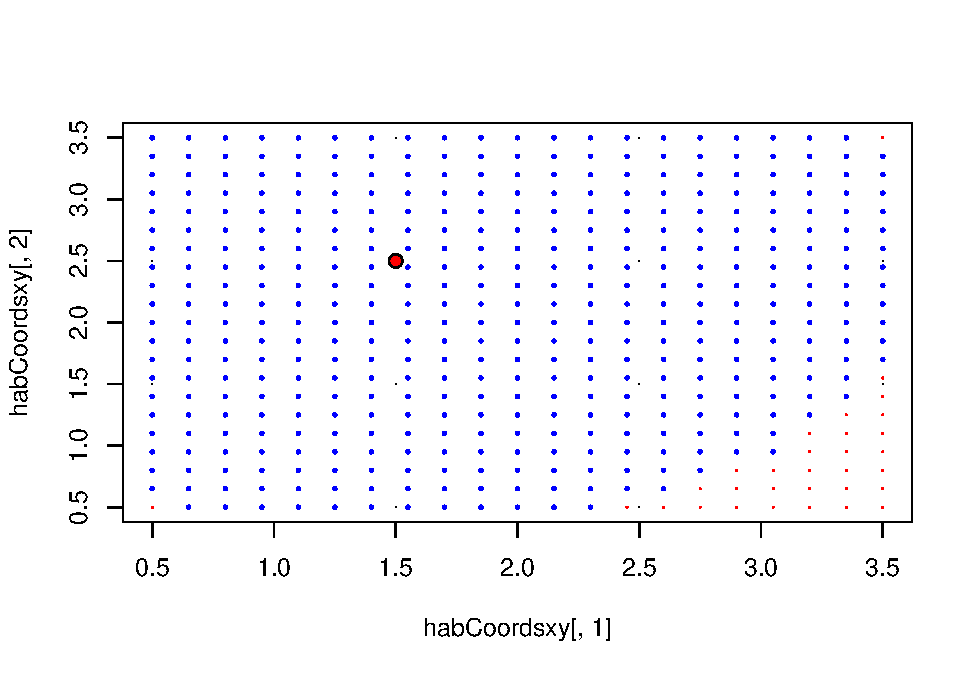
\includegraphics{InterruptionsPDF_files/figure-latex/4-1.pdf}

\begin{Shaded}
\begin{Highlighting}[]
\NormalTok{nimConstants}\OperatorTok{$}\NormalTok{maxNBDets <-}\StringTok{ }\NormalTok{DetectorIndexLESS}\OperatorTok{$}\NormalTok{maxNBDets}
\NormalTok{nimConstants}\OperatorTok{$}\NormalTok{y.maxDet <-}\StringTok{ }\KeywordTok{dim}\NormalTok{(DetectorIndexLESS}\OperatorTok{$}\NormalTok{habitatID)[}\DecValTok{1}\NormalTok{]}
\NormalTok{nimConstants}\OperatorTok{$}\NormalTok{x.maxDet <-}\StringTok{ }\KeywordTok{dim}\NormalTok{(DetectorIndexLESS}\OperatorTok{$}\NormalTok{habitatID)[}\DecValTok{2}\NormalTok{]}
\NormalTok{nimData}\OperatorTok{$}\NormalTok{detectorIndex<-}\StringTok{ }\NormalTok{DetectorIndexLESS}\OperatorTok{$}\NormalTok{detectorIndex}
\NormalTok{nimData}\OperatorTok{$}\NormalTok{habitatIDDet<-}\StringTok{ }\NormalTok{DetectorIndexLESS}\OperatorTok{$}\NormalTok{habitatID}

\NormalTok{nimData}\OperatorTok{$}\NormalTok{nDetectorsLESS <-}\StringTok{ }\NormalTok{DetectorIndexLESS}\OperatorTok{$}\NormalTok{nDetectorsLESS}
\NormalTok{nimConstants}\OperatorTok{$}\NormalTok{n.cellsSparse <-}\StringTok{ }\KeywordTok{dim}\NormalTok{(DetectorIndexLESS}\OperatorTok{$}\NormalTok{detectorIndex)[}\DecValTok{1}\NormalTok{]}
\NormalTok{nimConstants}\OperatorTok{$}\NormalTok{ResizeFactor <-}\StringTok{ }\NormalTok{DetectorIndexLESS}\OperatorTok{$}\NormalTok{ResizeFactor}
\NormalTok{nimConstants}\OperatorTok{$}\NormalTok{maxDist <-}\StringTok{ }\FloatTok{2.2}
\end{Highlighting}
\end{Shaded}

Last, we re-express the detection matrix y to reduce its size. We use a
new representation, where each row (corresponding to one individual)
contains the detector identification numbers (values of j) which
detected that individual.

A second matrix of identical dimension was also created, containing the
number of detections occurring at each detector. The second matrix would
be necessary for modelling non-binary detections.

\begin{Shaded}
\begin{Highlighting}[]
\CommentTok{### ==== 2. CREATE SPARSE MATRICES ====}

\NormalTok{SparseY <-}\StringTok{ }\KeywordTok{GetSparseY}\NormalTok{(nimData}\OperatorTok{$}\NormalTok{y)}


\CommentTok{# ADD TO NIMDATA}
\NormalTok{nimData}\OperatorTok{$}\NormalTok{y =}\StringTok{ }\NormalTok{SparseY}\OperatorTok{$}\NormalTok{y }\CommentTok{## Detection array }
\NormalTok{nimData}\OperatorTok{$}\NormalTok{yDets =}\StringTok{ }\NormalTok{SparseY}\OperatorTok{$}\NormalTok{yDets}
\NormalTok{nimData}\OperatorTok{$}\NormalTok{nbDetections =}\StringTok{ }\NormalTok{SparseY}\OperatorTok{$}\NormalTok{nbDetections}
\NormalTok{nimData}\OperatorTok{$}\NormalTok{trials =}\StringTok{ }\KeywordTok{rep}\NormalTok{(}\DecValTok{1}\NormalTok{, nimConstants}\OperatorTok{$}\NormalTok{n.detectors)}

\NormalTok{nimConstants}\OperatorTok{$}\NormalTok{nMaxDetectors =}\StringTok{ }\NormalTok{SparseY}\OperatorTok{$}\NormalTok{nMaxDetectors}
\end{Highlighting}
\end{Shaded}

\begin{Shaded}
\begin{Highlighting}[]
\CommentTok{## IV.NIMBLE RUN }
\NormalTok{model <-}\StringTok{ }\KeywordTok{nimbleModel}\NormalTok{(}\DataTypeTok{code =}\NormalTok{ modelCode,}
                     \DataTypeTok{constants =}\NormalTok{ nimConstants,}
                     \DataTypeTok{data =}\NormalTok{ nimData,}
                     \DataTypeTok{inits =}\NormalTok{ nimInits,}
                     \DataTypeTok{check =} \OtherTok{FALSE}\NormalTok{,}
                     \DataTypeTok{calculate =} \OtherTok{FALSE}\NormalTok{)}
\end{Highlighting}
\end{Shaded}

\begin{verbatim}
## defining model...
\end{verbatim}

\begin{verbatim}
## building model...
\end{verbatim}

\begin{verbatim}
## setting data and initial values...
\end{verbatim}

\begin{verbatim}
## checking model sizes and dimensions...
\end{verbatim}

\begin{verbatim}
## Warning in model$checkBasics(): Possible size/dimension mismatch amongst vectors
## and matrices in BUGS expression: sxy[i, 1:2, 1] ~ dbinomPPSingle(lowerCoords
## = lowerHabCoords[1:16, 1:2], upperCoords = upperHabCoords[1:16, 1:2],
## intensityWeights = mu[1:16], areAreas = 1, numWindows = 16, lower_ = -Inf,
## upper_ = Inf). Ignore this warning if the user-provided distribution has
## multivariate parameters with distinct sizes or if size of variable differs from
## sizes of parameters.
\end{verbatim}

\begin{verbatim}
## Warning in model$checkBasics(): Possible size/dimension mismatch
## amongst vectors and matrices in BUGS expression: sxy[i, 1:2, t] ~
## dbinomMNormSourcePPSingle(lowerCoords = lowerHabCoords[1:16, 1:2], upperCoords
## = upperHabCoords[1:16, 1:2], sourceCoords = sxy[i, 1:2, t - 1], normSD = tau,
## intensityWeights = mu[1:16], areAreas = 1, numWindows = 16, localEvalParam
## = -1, lower_ = -Inf, upper_ = Inf). Ignore this warning if the user-provided
## distribution has multivariate parameters with distinct sizes or if size of
## variable differs from sizes of parameters.
\end{verbatim}

\begin{verbatim}
## Warning in model$checkBasics(): Possible size/dimension mismatch amongst vectors
## and matrices in BUGS expression: y[i, 1:7, t] ~ dbin_LESSCachedAllSparse(pZero
## = lifted_p0_times_toggle_oBt_cB_L32[t], sxy = sxy[i, 1:2, t], sigma = sigma,
## nbDetections = nbDetections[i, t], yDets = yDets[i, 1:7, t], detector.xy
## = detector.xy[1:441, 1:2], trials = trials[1:441], detectorIndex =
## detectorIndex[1:16, 1:410], nDetectorsLESS = nDetectorsLESS[1:16], ResizeFactor
## = 1, maxNBDets = 410, habitatID = habitatIDDet[1:4, 1:4], maxDist = 2.2,
## indicator = lifted_z_oBi_comma_t_cB_eq__eq_2_L32[i, t], lower_ = -Inf, upper_
## = Inf). Ignore this warning if the user-provided distribution has multivariate
## parameters with distinct sizes or if size of variable differs from sizes of
## parameters.
\end{verbatim}

\begin{verbatim}
##  This model is not fully initialized. This is not an error. To see which variables are not initialized, use model$initializeInfo(). For more information on model initialization, see help(modelInitialization).
## model building finished.
\end{verbatim}

\begin{Shaded}
\begin{Highlighting}[]
\NormalTok{cmodel <-}\StringTok{ }\KeywordTok{compileNimble}\NormalTok{(model)}
\end{Highlighting}
\end{Shaded}

\begin{verbatim}
## compiling... this may take a minute. Use 'showCompilerOutput = TRUE' to see C++ compilation details.
## compilation finished.
\end{verbatim}

\begin{Shaded}
\begin{Highlighting}[]
\NormalTok{cmodel}\OperatorTok{$}\KeywordTok{calculate}\NormalTok{()}
\end{Highlighting}
\end{Shaded}

\begin{verbatim}
## [1] -19082.62
\end{verbatim}

\begin{Shaded}
\begin{Highlighting}[]
\NormalTok{MCMCconf <-}\StringTok{ }\KeywordTok{configureMCMC}\NormalTok{(}\DataTypeTok{model =}\NormalTok{ model,}
                          \DataTypeTok{monitors =} \KeywordTok{c}\NormalTok{(params),}
                          \DataTypeTok{control =} \KeywordTok{list}\NormalTok{(}\DataTypeTok{reflective =} \OtherTok{TRUE}\NormalTok{, }\DataTypeTok{adaptScaleOnly =} \OtherTok{TRUE}\NormalTok{),}
                          \DataTypeTok{useConjugacy =} \OtherTok{FALSE}\NormalTok{)}
\NormalTok{MCMC <-}\StringTok{ }\KeywordTok{buildMCMC}\NormalTok{(MCMCconf)}
\NormalTok{cMCMC <-}\StringTok{ }\KeywordTok{compileNimble}\NormalTok{(MCMC, }\DataTypeTok{project =}\NormalTok{ model, }\DataTypeTok{resetFunctions =} \OtherTok{TRUE}\NormalTok{)}
\end{Highlighting}
\end{Shaded}

\begin{verbatim}
## compiling... this may take a minute. Use 'showCompilerOutput = TRUE' to see C++ compilation details.
## compilation finished.
\end{verbatim}

\begin{Shaded}
\begin{Highlighting}[]
\KeywordTok{set.seed}\NormalTok{(}\DecValTok{0}\NormalTok{)}
\NormalTok{myNimbleOutput <-}\StringTok{ }\KeywordTok{runMCMC}\NormalTok{(}\DataTypeTok{mcmc =}\NormalTok{ cMCMC,}
                          \DataTypeTok{nburnin =}\NormalTok{ nburnin,}
                          \DataTypeTok{niter =}\NormalTok{ niter, }
                          \DataTypeTok{nchains =}\NormalTok{ nchains, }
                          \DataTypeTok{samplesAsCodaMCMC =} \OtherTok{TRUE}\NormalTok{)}
\end{Highlighting}
\end{Shaded}

\begin{verbatim}
## running chain 1...
\end{verbatim}

\begin{verbatim}
## |-------------|-------------|-------------|-------------|
## |-------------------------------------------------------|
\end{verbatim}

\hypertarget{v.plot-output}{%
\subsection{V.PLOT OUTPUT}\label{v.plot-output}}

\begin{Shaded}
\begin{Highlighting}[]
\CommentTok{# N}
\ControlFlowTok{for}\NormalTok{(t }\ControlFlowTok{in} \DecValTok{1}\OperatorTok{:}\NormalTok{n.occasions)\{ }
  \KeywordTok{PlotParams}\NormalTok{(myNimbleOutput,}
             \DataTypeTok{params=} \KeywordTok{paste}\NormalTok{(}\StringTok{"N["}\NormalTok{,t,}\StringTok{"]"}\NormalTok{, }\DataTypeTok{sep=}\StringTok{""}\NormalTok{),}
             \DataTypeTok{sim.values=}\NormalTok{Pop.Compo[[}\DecValTok{2}\NormalTok{]][t])}
\NormalTok{\}}
\end{Highlighting}
\end{Shaded}

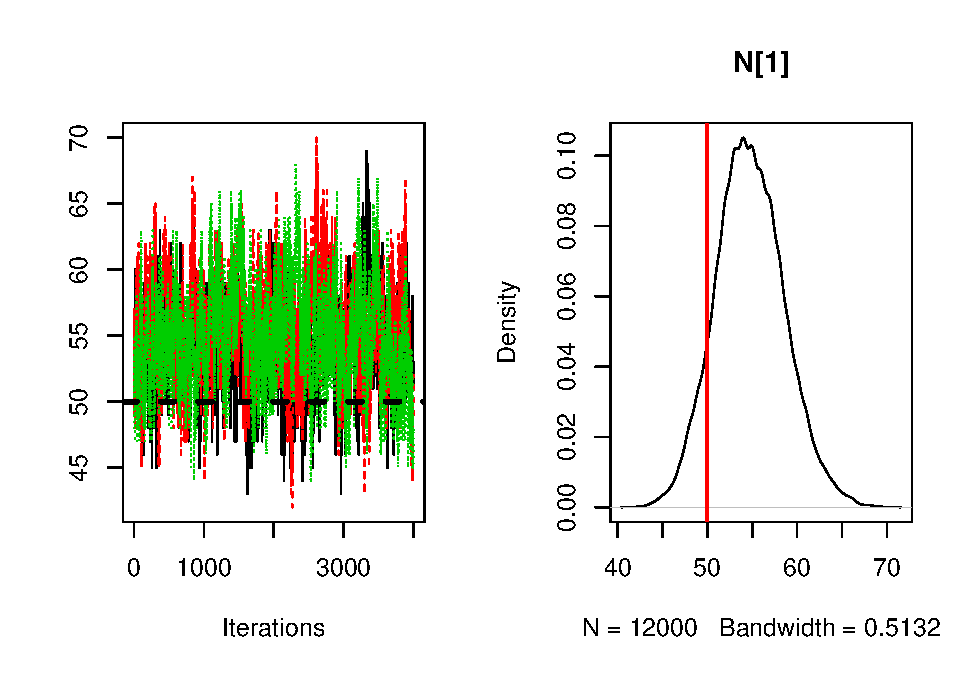
\includegraphics{InterruptionsPDF_files/figure-latex/PLOT-1.pdf}
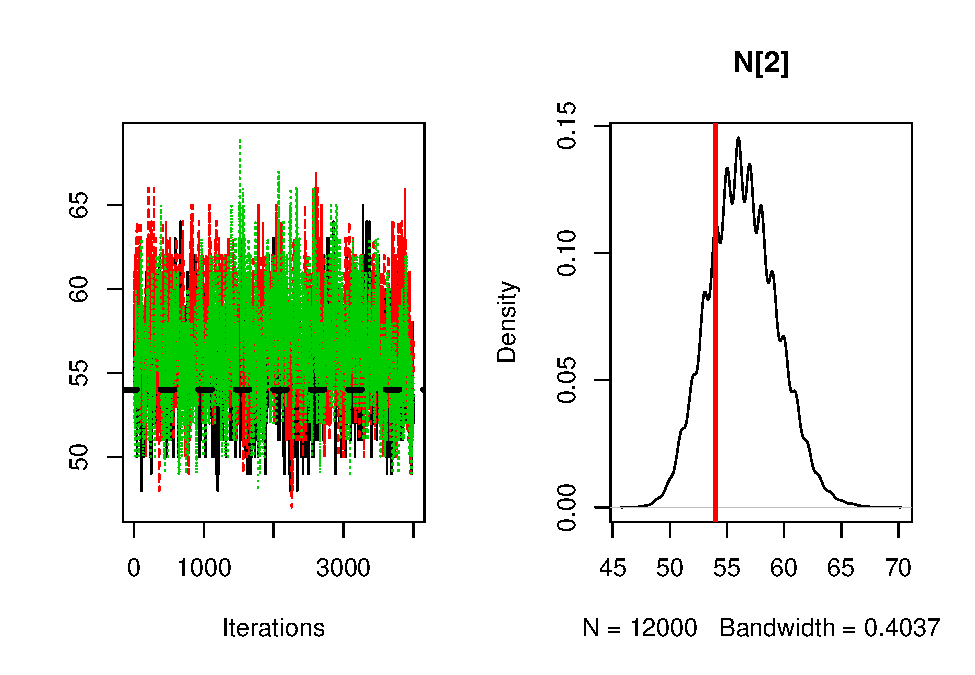
\includegraphics{InterruptionsPDF_files/figure-latex/PLOT-2.pdf}
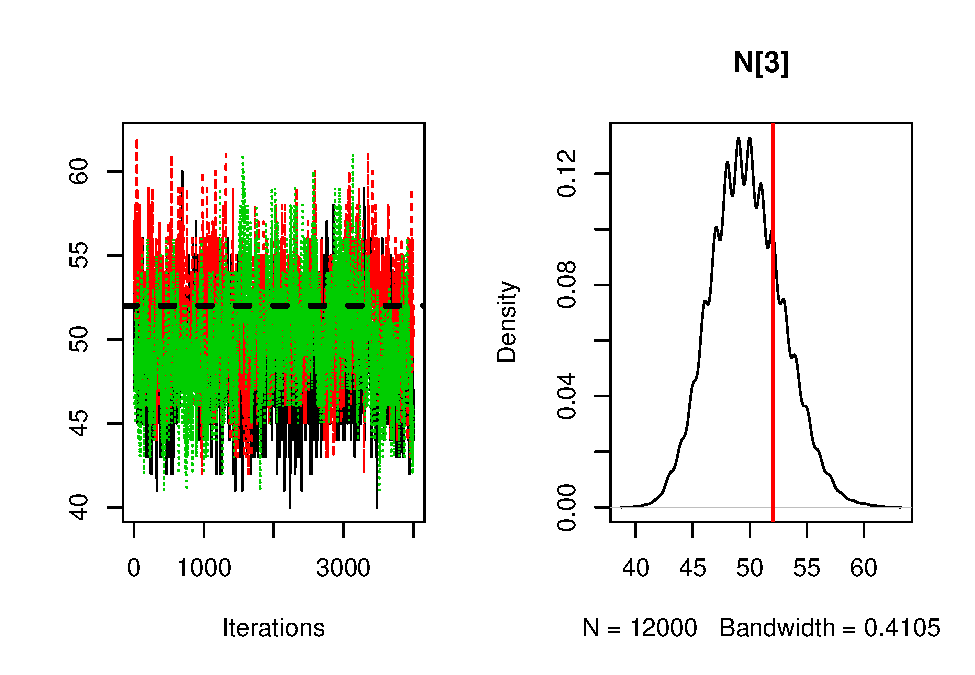
\includegraphics{InterruptionsPDF_files/figure-latex/PLOT-3.pdf}
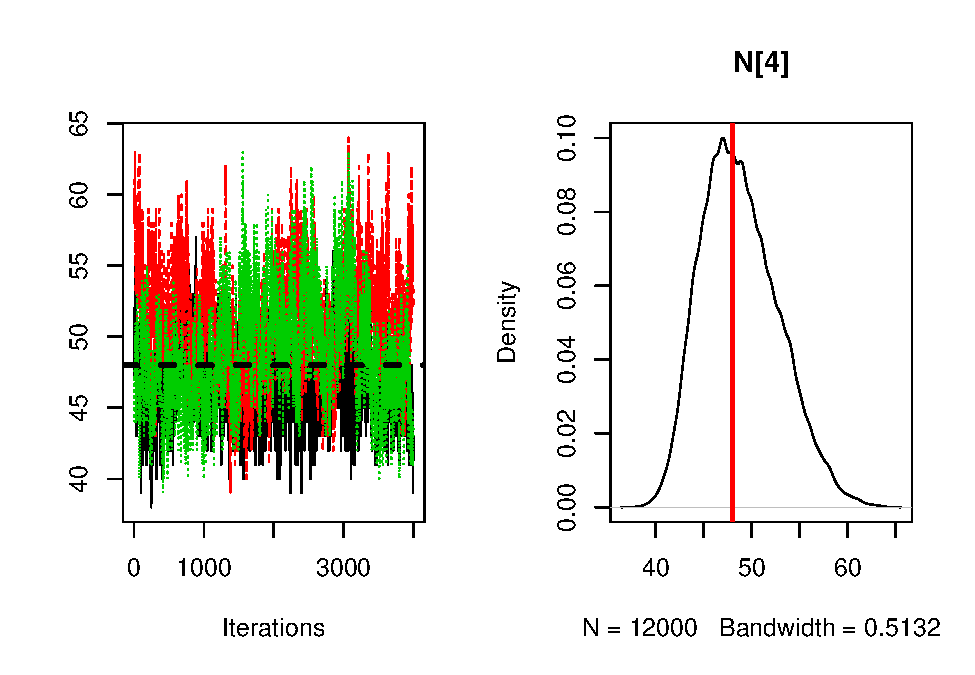
\includegraphics{InterruptionsPDF_files/figure-latex/PLOT-4.pdf}
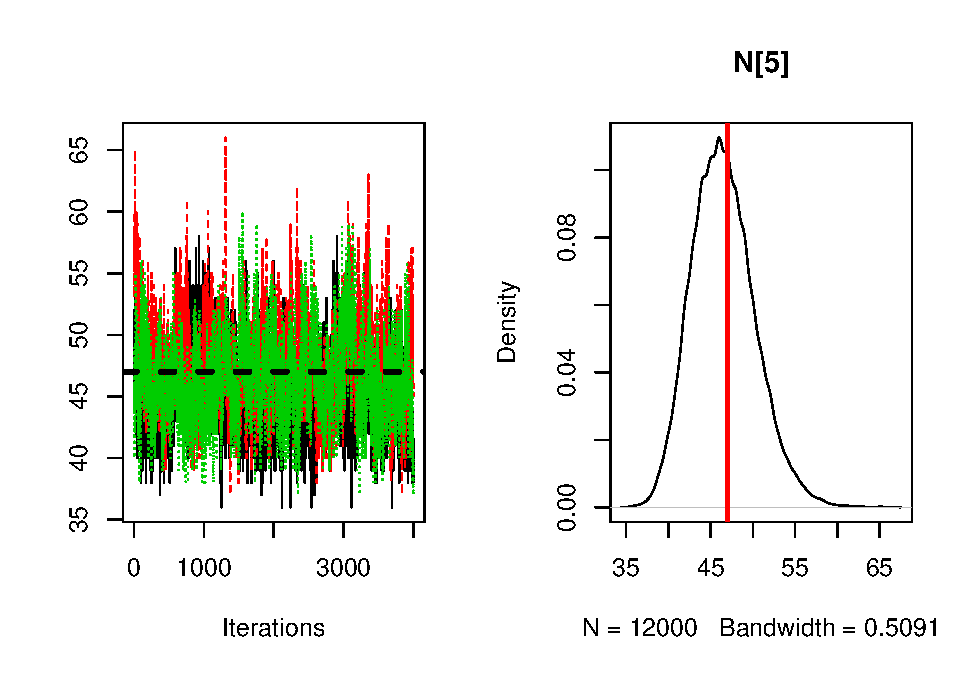
\includegraphics{InterruptionsPDF_files/figure-latex/PLOT-5.pdf}

\begin{Shaded}
\begin{Highlighting}[]
\CommentTok{# SIGMA}
\KeywordTok{PlotParams}\NormalTok{(myNimbleOutput, }\DataTypeTok{params=} \StringTok{"sigma"}\NormalTok{, }\DataTypeTok{sim.values=}\NormalTok{sigma}\OperatorTok{/}\KeywordTok{res}\NormalTok{(r))}
\end{Highlighting}
\end{Shaded}

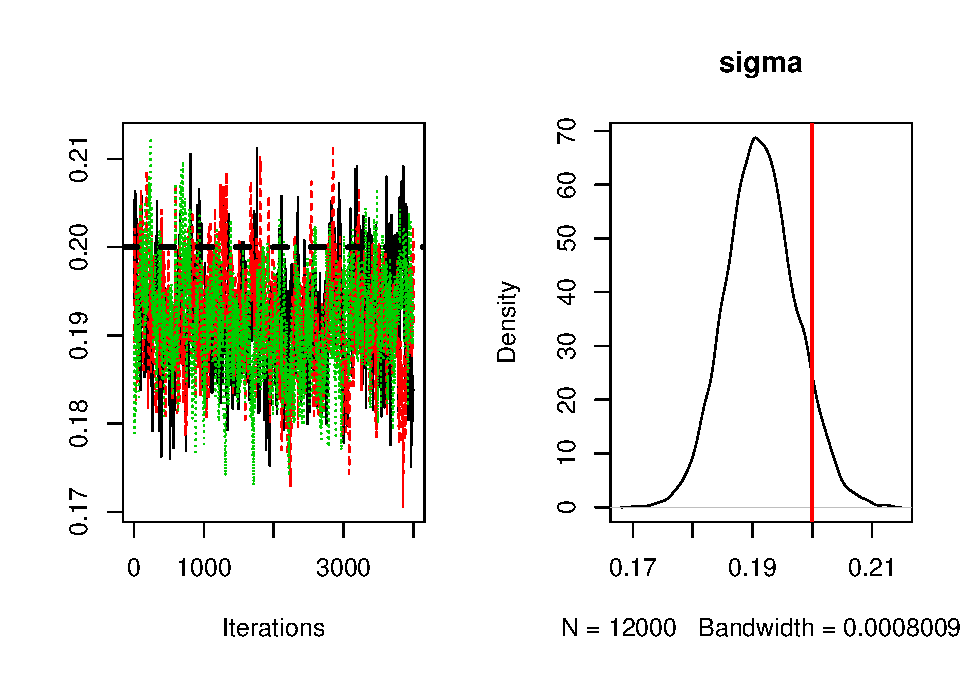
\includegraphics{InterruptionsPDF_files/figure-latex/PLOT-6.pdf}

\begin{Shaded}
\begin{Highlighting}[]
\CommentTok{# p0}
\KeywordTok{PlotParams}\NormalTok{(myNimbleOutput, }\DataTypeTok{params=} \StringTok{"p0"}\NormalTok{, }\DataTypeTok{sim.values=}\NormalTok{p0)}
\end{Highlighting}
\end{Shaded}

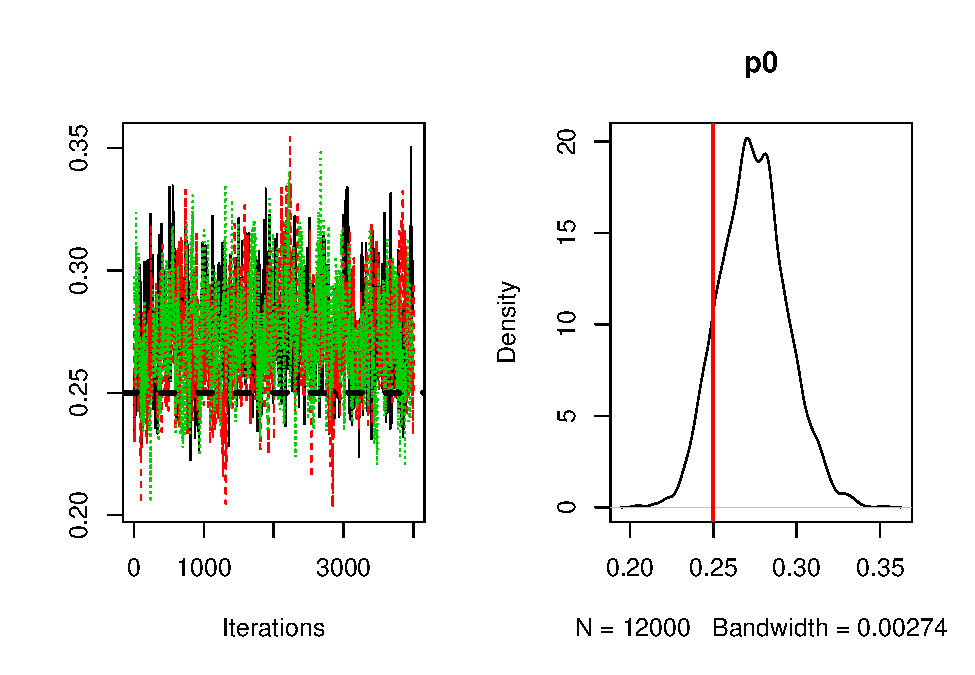
\includegraphics{InterruptionsPDF_files/figure-latex/PLOT-7.pdf}

\begin{Shaded}
\begin{Highlighting}[]
\CommentTok{# tau}
\KeywordTok{PlotParams}\NormalTok{(myNimbleOutput, }\DataTypeTok{params=} \StringTok{"tau"}\NormalTok{, }\DataTypeTok{sim.values=}\NormalTok{tau}\OperatorTok{/}\KeywordTok{res}\NormalTok{(r))}
\end{Highlighting}
\end{Shaded}

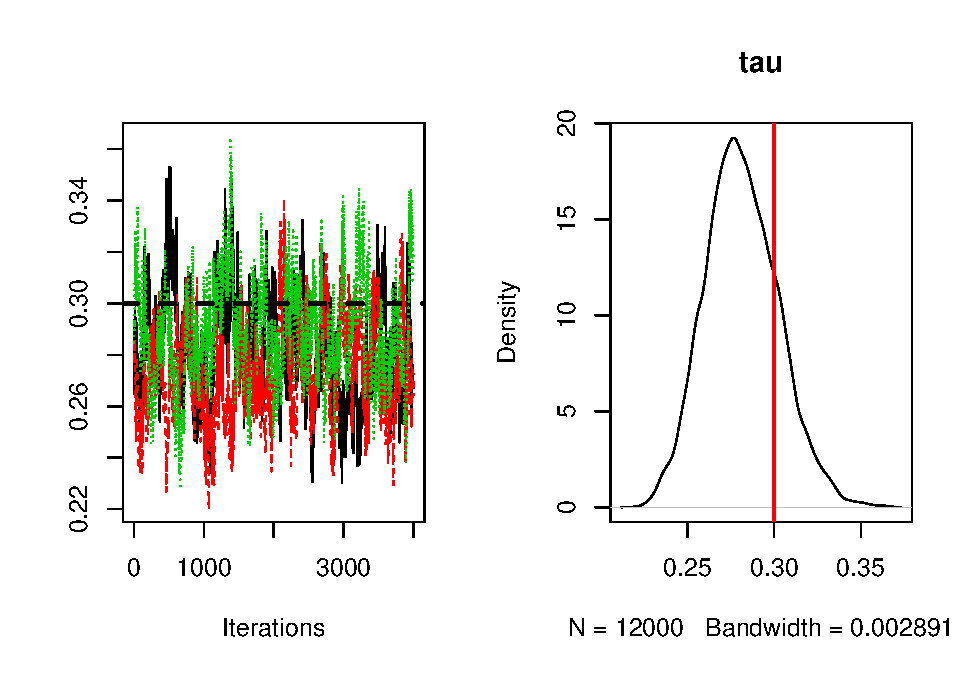
\includegraphics{InterruptionsPDF_files/figure-latex/PLOT-8.pdf}

\begin{Shaded}
\begin{Highlighting}[]
\CommentTok{# phi}
\KeywordTok{PlotParams}\NormalTok{(myNimbleOutput, }\DataTypeTok{params=} \StringTok{"phi"}\NormalTok{, }\DataTypeTok{sim.values=}\NormalTok{phi)}
\end{Highlighting}
\end{Shaded}

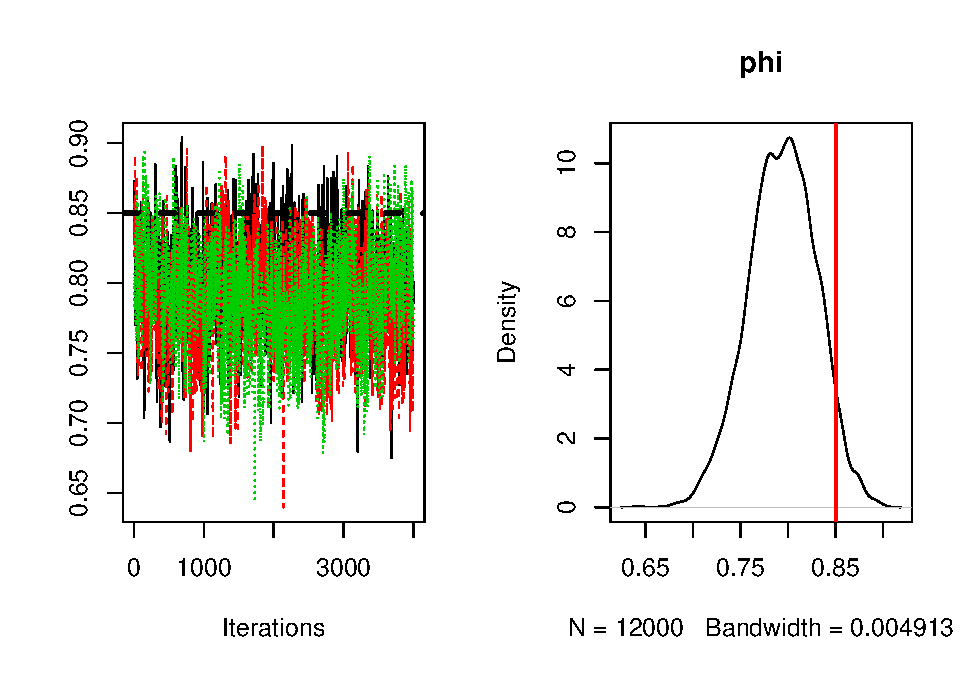
\includegraphics{InterruptionsPDF_files/figure-latex/PLOT-9.pdf}

\begin{Shaded}
\begin{Highlighting}[]
\CommentTok{# rho}
\KeywordTok{PlotParams}\NormalTok{(myNimbleOutput, }\DataTypeTok{params=} \StringTok{"rho"}\NormalTok{, }\DataTypeTok{sim.values=}\NormalTok{rho)}
\end{Highlighting}
\end{Shaded}

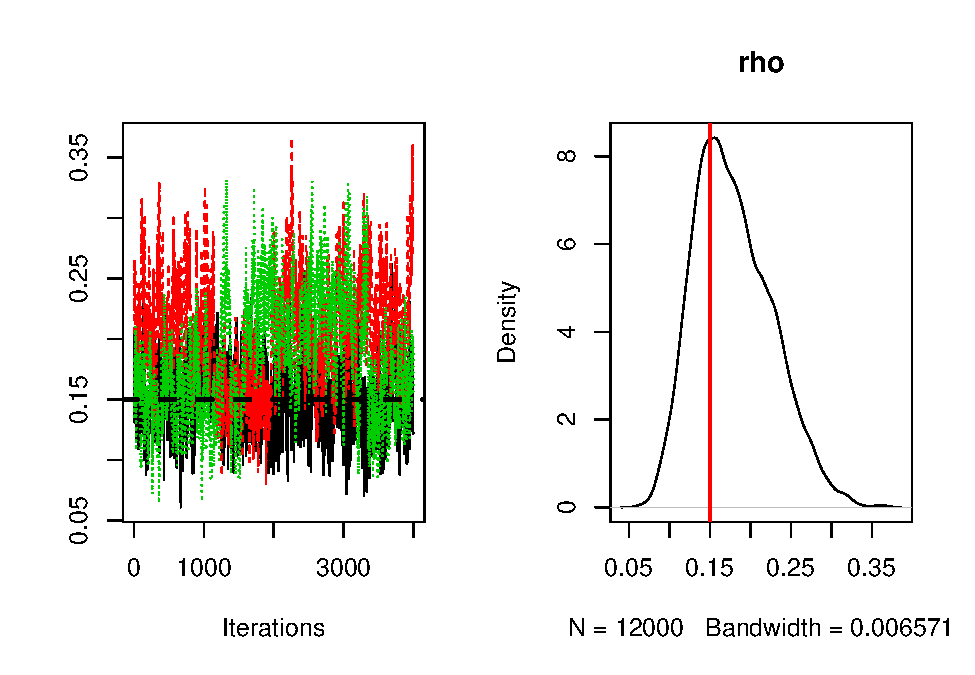
\includegraphics{InterruptionsPDF_files/figure-latex/PLOT-10.pdf}

\hypertarget{references}{%
\subsection*{REFERENCES}\label{references}}
\addcontentsline{toc}{subsection}{REFERENCES}

\hypertarget{refs}{}
\leavevmode\hypertarget{ref-Milleret2019}{}%
Milleret, C., P. Dupont, C. Bonenfant, H. Broseth, O. Flagstad, C.
Sutherland, and R. Bischof. 2019. ``A Local Evaluation of the Individual
State Space to Scale up Bayesian Spatial Capture Recapture.''
\emph{Ecology and Evolution} 9 (1): 352--63.
\url{https://doi.org/10.1002/ece3.4751}.

\leavevmode\hypertarget{ref-NIMBLE}{}%
NIMBLE Development Team. 2019. \emph{NIMBLE: MCMC, Particle Filtering,
and Programmable Hierarchical Modeling}.
https://cran.r-project.org/package=nimble:
https://cran.r-project.org/package=nimble.
\url{https://doi.org/http://doi.org/10.5281/zenodo.1211190}.

\leavevmode\hypertarget{ref-deValpine2017}{}%
Valpine, P. de, D. Turek, C. J. Paciorek, C. Anderson-Bergman, D. T.
Lang, and R. Bodik. 2017. ``Programming with Models: Writing Statistical
Algorithms for General Model Structures with Nimble.'' \emph{Journal of
Computational and Graphical Statistics} 26 (2): 403--13.

\end{document}
